%&format

% The above line adds the format that can be compiled with the following command:
% pdflatex -ini -jobname="format" "&pdflatex" mylatexformat.ltx """Phd-Thesis-Format.tex"""

%-------------------------------------------------------------------------------
% Technical things
%-------------------------------------------------------------------------------
% Include all chapters/sections so the references are present
\includeonly{chapters/objects}



%-------------------------------------------------------------------------------
% Content
%-------------------------------------------------------------------------------
\begin{document}

% \maketitle

\tableofcontents

% List of to-do notes.
\listoftodos

% -------------------------------------------------------------------------------
\chapter{Introduction}
\label{sec:intro}

% \Rnote{}{Test reminder todo note}
% \Qinote{}{Test inline question todo note}
% \TDnote{}{Test TODO todo note}

%-------------------------------------------------------------------------------

Place your introduction here.

\chapter{Theoretical Background}
\label{chap:theory}
\section{The Standard Model of Particle Physics}
\section{The anatomy of Proton-Proton Collision Events}
\section{Higgs Boson Physics}


% %-------------------------------------------------------------------------------

\chapter{The ATLAS Experiment at the Large Hadron Collider}
\label{chap:experiment}
%To test the theoretical predictions of the Standard Model, huge experimental setups with unprecedented size and complexity are required.
The ATLAS experiment~\cite{PERF-2007-01} is a multipurpose detector that measures the particle-particle collisions produced by the \emph{Large Hadron Collider} (LHC)~\cite{Evans:2008zzb} with extreme precision. It is designed to measure a broad range of physics processes, with a focus on providing more insight into the Higgs boson.
The LHC is the world's most powerful particle accelerator to date. It remains the most recent large-scale upgrade to the accelerator complex at CERN, the \emph{European Organization for Nuclear Research}, and produces collision events at unprecedented energies.
This chapter first provides an overview of the LHC, followed by a detailed description of the various aspects of the ATLAS experiment.

\section{The Large Hadron Collider}
%The two major technical components are \emph{radiofrequency cavities} (RF cavities) with oscillating electromagnetic fields to accelerate the particles as well as organizing them in so-called \emph{bunches}\footnote{RF cavities oscillate at a given frequency. Particles arriving early (late), will be decelerated (accelerated) so that the particles are kept together in discrete packages called bunches.} and magnet systems to bend, steer, and focus the particles' trajectories. The peak particle energy reached by a hadron collider is thereby limited by the maximum field strength of the bending magnets.
The LHC was designed and built for more than two decades starting in the early 1980s by more than $10000$ international researchers, engineers, and technicians from more than $100$ different countries.
The LHC is located in a near-circular tunnel\footnote{The same tunnel was used by the former LEP collider~\cite{LEPDesignReport}.} an average of \SI{100}{\m} below the France-Switzerland border close to Geneva (Switzerland). It has a circumference of \SI{26.7}{\km} and in its main mode of operation collides protons\footnote{The LHC also produces heavy-ion collisions in dedicated running periods} with a centre-of-mass energy of $\comEn = \SI{13}{\TeV}$\footnote{The LHC design centre-of-mass energy is $\comEn = \SI{14}{\TeV}$.}.
The protons are accelerated with 16 \emph{radiofrequency cavities}, that have oscillating electromagnetic fields and group the protons in \emph{bunches}\footnote{The radiofrequency cavities oscillate at a design frequency of \SI{400}{\mega\hertz}. The particles that arrive early (late), are decelerated (accelerated) so that the particles are kept together in discrete packages called bunches.}.
These bunches occupy two separate but nearby rings to form counter-rotating particle beams.
The LHC is designed to contain a maximum of 2808 bunches that are separated by a bunch spacing of \SI{25}{\ns}. Each bunch consists of about \SI{e11}{protons} which results in a design instantaneous luminosity of $\instLumi = \SI{e34}{\per\cm\per\s}$.\footnote{The machine and beam parameters of the LHC can vary between different data-taking cycles. More details can be found in \cref{sec:run-2-data-taking}.}
More than 1200 superconducting dipole magnets are used to force the particle beams on a curved trajectory.
They are designed to reach field strengths of up to \SI{8.33}{\tesla}, enabling the unprecedented collision energies\footnote{The peak particle energy reached by a hadron collider is limited by the maximum field strength of the bending magnets.}. More than 400 quadrupole magnets are used to focus the beams and increase the particle density within each bunch, which is especially important before the beams collide at any of the four main \emph{interaction points} (IPs). Each IP is surrounded by large detector systems that are optimized and designed for different physics objectives.
The ATLAS\footnote{A Toroidal Lhc ApparatuS} and CMS\footnote{Compact Muon Solenoid}~\cite{CMS-TDR-08-001} experiments are multipurpose detectors, designed to measure a large variety of physics processes. The LHCb\footnote{Large Hadron Collider beauty} experiment~\cite{1748-0221-3-08-S08005} is dedicated to measuring processes that involve $b$-quarks and ALICE\footnote{A Large Ion Collider Experiment}~\cite{1748-0221-3-08-S08002} focuses on the analysis of heavy-ion collisions.\footnote{There are other smaller experiments operating at the LHC: the TOTEMd (Total Elastic and Diffractive Cross Section Measurement)~\cite{1748-0221-3-08-S08007} and LHCf (Large Hadron Collider forward)~\cite{1748-0221-3-08-S08006} experiments study scattering processes close to the beam line and the MoEDAL (Monopole and Exotics Detector at the LHC) experiment~\cite{1742-6596-631-1-012014} is dedicated to the search for magnetic monopoles.}

Before the protons enter the LHC, they pass through a series of smaller accelerators. A schematic of the entire accelerator complex is shown in \cref{fig:accelerator-complex}.
The protons are extracted by ionising hydrogen atoms and first accelerated in the linear accelerator \emph{Linac2} (Linear accelerator 2)\footnote{Starting in 2020, Linac2 will be replaced by a new linear accelerator, Linac4 (Linear accelerator 4). More information can be found in \ccite{CERN-AB-2006-084}.}. Three synchrotrons follow: the \emph{BOOSTER} (Proton Synchrotron Booster), the \emph{PS} (Proton Synchrotron), and the \emph{SPS} (Super Proton Synchrotron).
They have an increasingly larger circumference and gradually increase the energy of the proton beams.
The proton beams from the SPS are finally injected into the LHC with an energy of $450\,\GeV$. The filling and ramp-up phases until stable beams are brought to collision at their final energies take around 45 minutes. The experiments at the LHC record the collision events for ideally about 8-10 hours or more, until the intensity of the beams becomes too low, making it more efficient to dump the beam and start a new cycle.

The operation of the LHC is broken down into different runs that last several years with differing running conditions.
\Cref{tab:lhc-lumi-overview-years} shows basic characteristics of the $pp$ collisions produced in so-called \RunOne and \RunTwo of the LHC, that occured between 2011-2012 and 2015-2018, respectively. After a technical shutdown between 2018 and 2022, the LHC is expected to continue to operate with \RunThr at a centre-of-mass energy \TDnote{of}{check again later} $\sqrt{s} = \SI{13.6}{\TeV}$.
Details on the \RunTwo data taking period and the performance of the ATLAS data acquisition are given in \cref{sec:run-2-data-taking}.

\FloatBarrier

\begin{table}[t]
  \centering
  \begin{tabular}{l | c | rr}
    \toprule
                             & Year      & \comEn [\TeV] & \intLumi [\ifb] \\
    \midrule
    \multirow{2}{*}{\RunOne} & 2011      & 7             & 5.5             \\
                             & 2012      & 8             & 22.8            \\
    \midrule
    \multirow{4}{*}{\RunTwo} & 2015      & 13            & 4.2             \\
                             & 2016      & 13            & 38.5            \\
                             & 2017      & 13            & 50.2            \\
                             & 2018      & 13            & 63.3            \\
    \midrule
    Full \RunTwo             & 2015-2018 & 13            & 156.2           \\
    \bottomrule
  \end{tabular}
  \caption{
    Summary of the centre-of-mass energy and integrated luminosity delivered by the LHC in $pp$ collisions during \RunOne and \RunTwo.}
  \label{tab:lhc-lumi-overview-years}
\end{table}

% Taken from \ccite{PublicLumiResults,PublicLumiResultsRun1}.




\begin{figure}
    %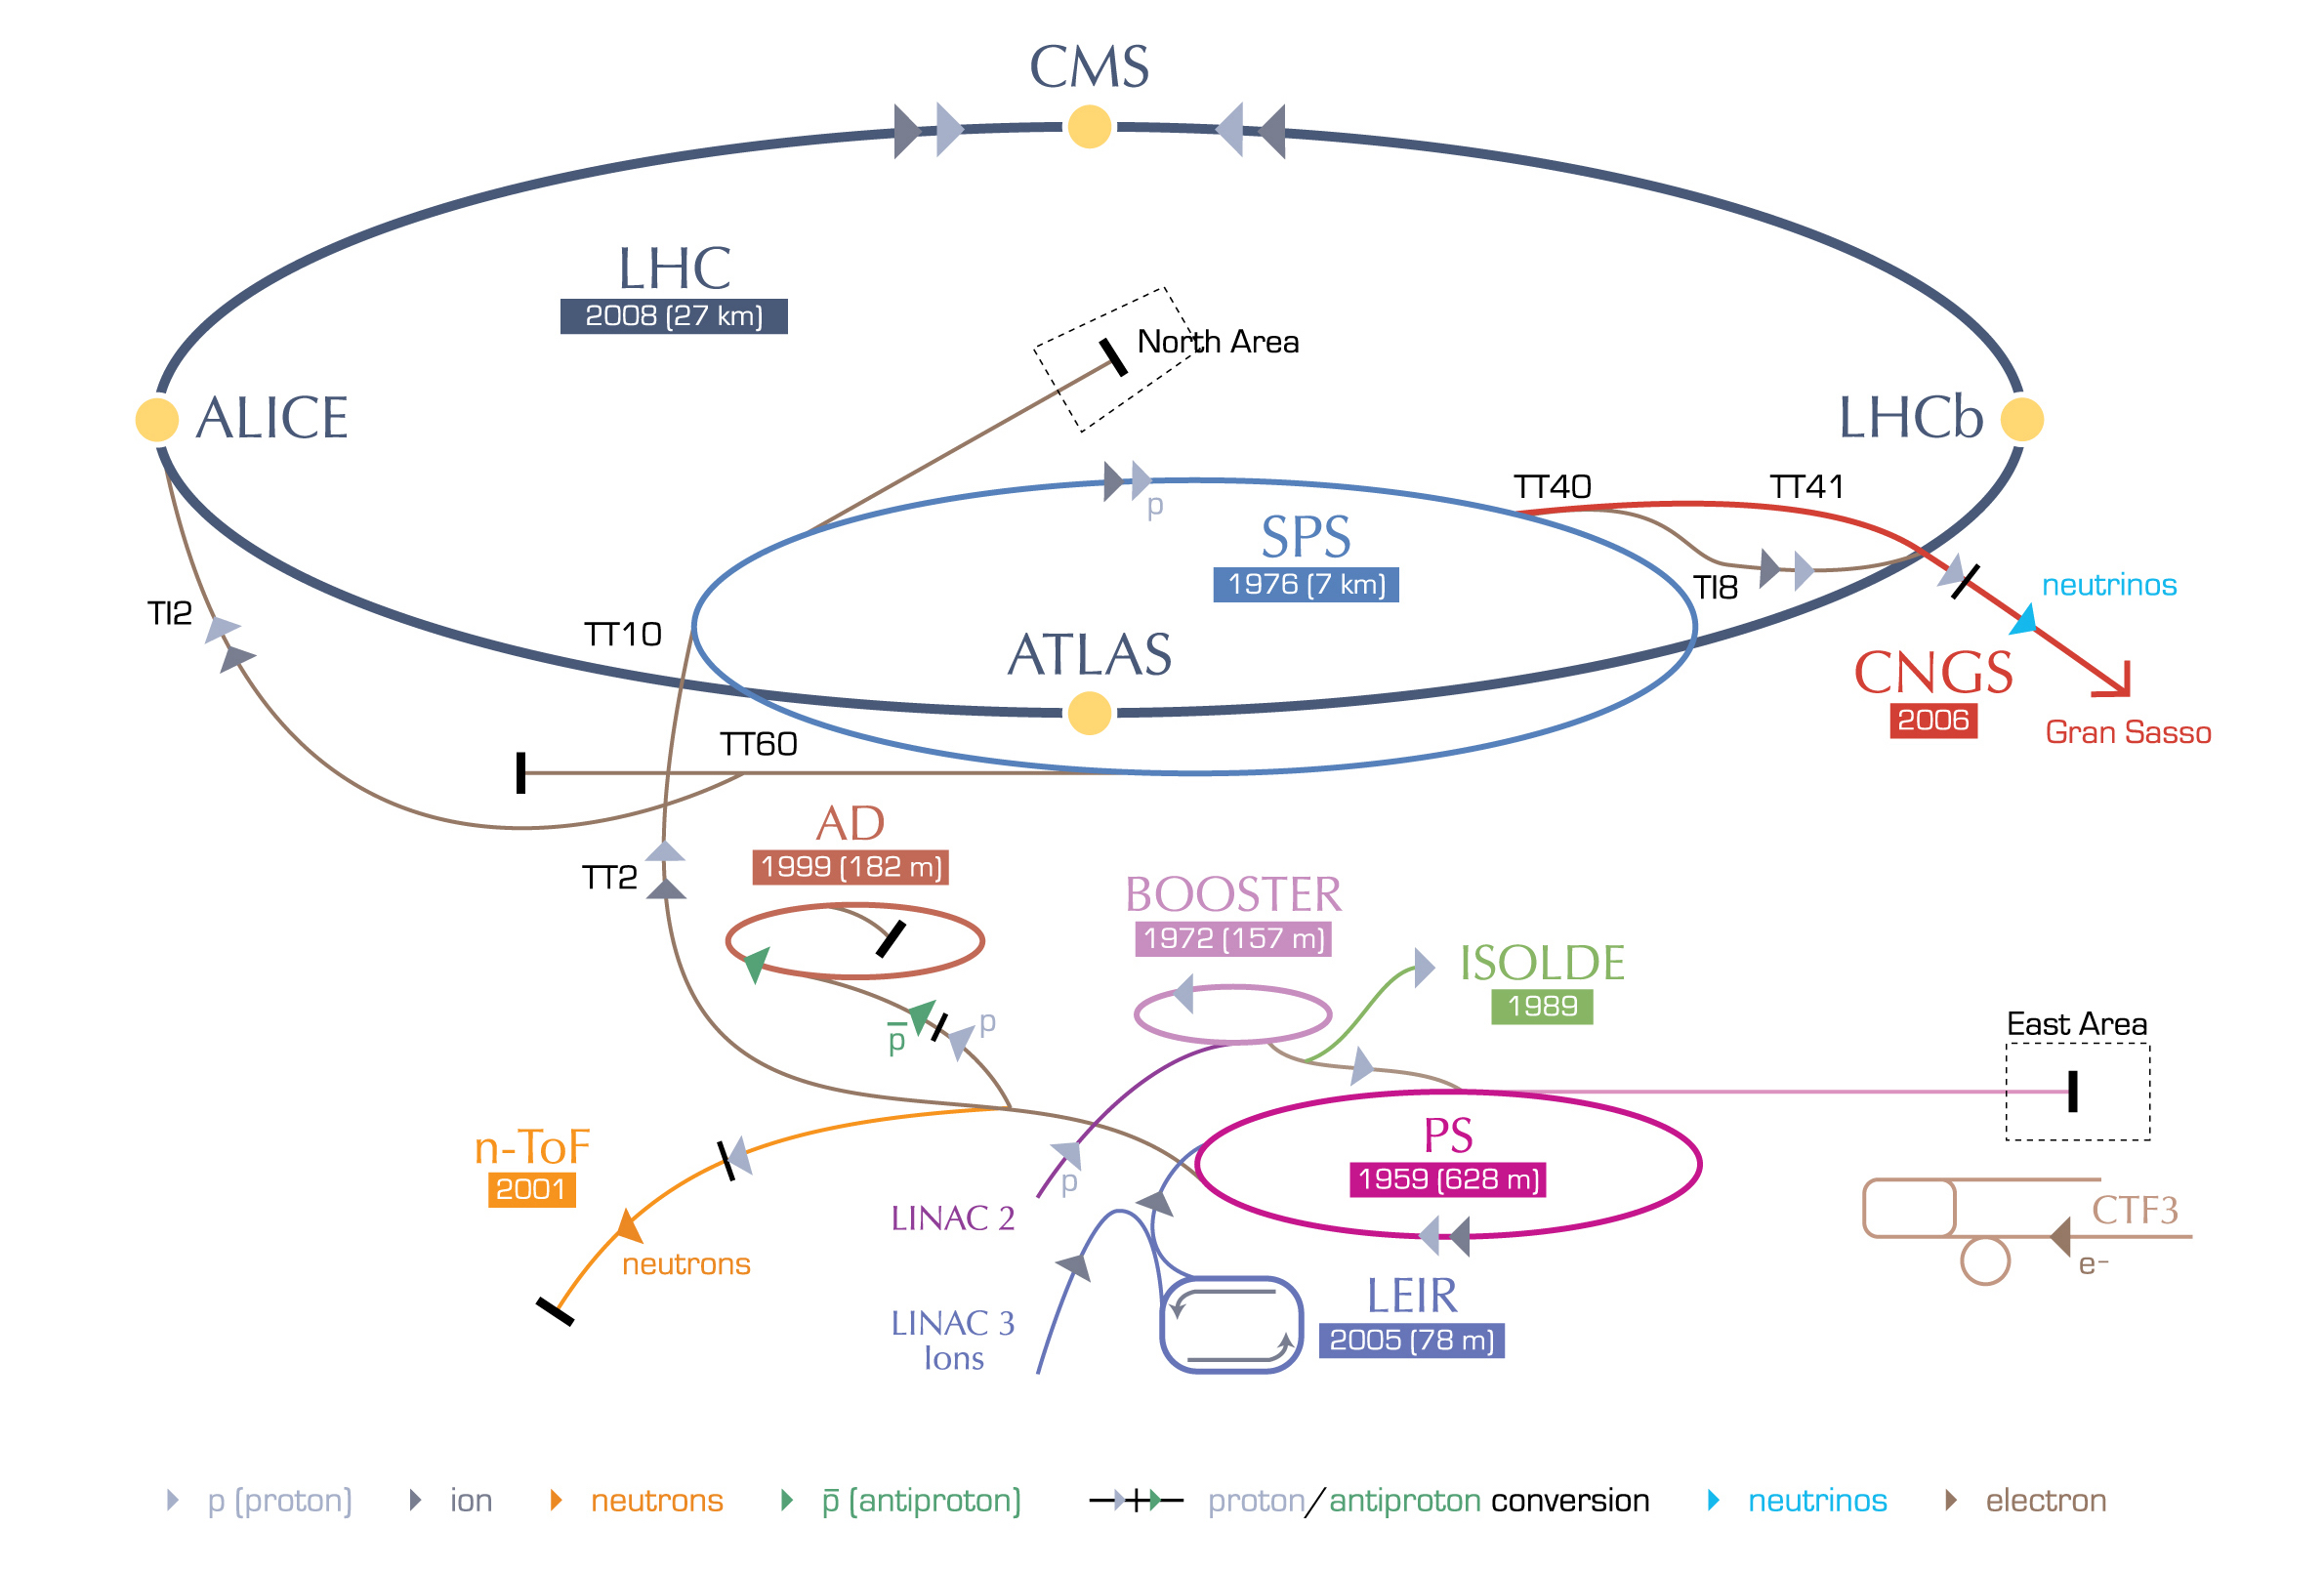
\includegraphics{figures/experiment/accelerator-complex.jpg}
    \newImageResize{figures/experiment/accelerator-complex.jpg}
    \caption{Illustration of the accelerator complex at CERN, including the Linac2, BOOSTER, PS, and SPS that serve as pre-accelerators before the protons are injected into the LHC. Adapted from \ccite{Christiane:1260465}.}
    \label{fig:accelerator-complex}
\end{figure}







\section{The ATLAS Experiment}
The ATLAS experiment is operated by a community of about 3000 scientific authors from 181 institutions and 41 countries~\cite{AtlasCollab}, making it one of the largest scientific collaborations in the world.
This section first provides an overview of the detection principles used to measure the various products of the $pp$ collision events and gives detailed information on the detector setup thereafter.

\subsection{Detection principles}
\label{subsec:measurement-principles}
Different types of particles, such as electrons, muons, or hadrons, originate from the $pp$ collisions and are measured in the ATLAS detector using two main methods: by detecting their trajectories, a method known as \emph{tracking}, and by measuring their energy via total absorption, a principle known as \emph{calorimetry}.

\subsubsection{Tracking}
%To reconstruct the trajectories of charged particles in the ATLAS detector, 
Tracks from charged particles can be reconstructed by measuring discrete space points and recognizing patterns.
The mostly non-destructive space point measurements are provided by detecting the signals (or \emph{hits}) left by traversing charged particles in finely segmented detector layers with known position. Different techniques are used in the ATLAS detector for this purpose:
\paragraph{Silicon semiconductor sensors} detect electron-hole pairs that are created in a p-n junction when a charged particle traverses the material. They can be segmented very finely and thus deliver precise spatial measurements.
\paragraph{Gas filled detectors} measure the current induced after a charged particle ionises a gas via a wire connected at high voltage. The detectors consist of tubes or chambers with different arrangements of electrodes. Their main advantage is a low material cost which makes them useful for covering large areas. \\
% \paragraph{Transition radiation detectors} are based on gaseous ionisation detectors and additionally measure the transition radiation from charged particles that traverse through material with different dielectric constants. The amount of transition radiation is sensitive to the Lorentz factor, which in combination with a momentum measurement provides the ability to measure the mass of a charged particle. This is useful input for particle identification. \\
\newline
To enable momentum measurements of charged particles, the tracking devices are immersed in magnetic fields that force the particles on a curved path. Their momenta can be determined from the radius of curvature of their reconstructed tracks. The resolution of the momentum measurement deteriorates linearly as the particle momentum increases.
%The following types of tracking devices are used in the ATLAS detector:
%The tracking devices are immersed in magnetic fields that force the charged particles on a curved path, allowing their momenta to be measured through the radius of their reconstructed tracks. 
% to bend the charged particles' trajectories. 
% This allows to measure the momentum of charged particles through the radius of their reconstructed track.

\subsubsection{Calorimetry}
%\emph{Calorimetry} can be defined as the detection principle to measure the energy of physics objects by fully absorbing them in blocks of instrumented material, called calorimeters.

Calorimeters measure the energy of particles by fully absorbing them and transferring their energy to electrical signals.
The ATLAS calorimeter is a so-called \emph{sampling calorimeter} where each of these tasks is handled by a dedicated material.
Layers of high-density \emph{passive material} are predominantly responsible for stopping the particles and are alternated with layers of \emph{active material} that focus on measuring the signals induced by the particles.
The total signal measured is proportional to the energy of the incident particle.

% comment from Mike (should be incorporated now!)
% This description is not strictly correct. It implies that the passive material stops the particles, which is true only as a whole. To be precise, there is also energy loss in the active material but of course much less.
% It is better to say that the absorber initiates showers, which are detected in the active layers. I see that you do this below.
% We can talk about how to re-word this if you want but I would rather you do it.


% Layers of \emph{passive material} stop the particles by initiating a process of repeated interactions with the detector material. They are alternated with layers of \emph{active material} that measure the signals deposited by the particles participating in the shower. 
% The ATLAS detector uses so-called \emph{sampling calorimeters} that comprise alternating layers of \emph{active material}, to actively measure the signals of the showering particles, and highly-dense \emph{passive material}, to initiate the showering and stop the particles.
\paragraph{Calorimeter showers}\mbox{}\\
As an incident particle interacts with the passive layers, a cascade of secondary particles forms.
Each secondary particle carries a fraction of the original energy and itself interacts with the calorimeter. This results in the formation of a \emph{calorimeter shower} that consists of particles with gradually decreasing energy as the shower evolves.
A distinction is made between \emph{electromagnetic showers} and \emph{hadronic showers}.

% The incident particles interact with the absorbers through several mechanisms which results in cascades of secondary particles known as \emph{showers}. 
Electromagnetic showers are initiated by electrons, positrons, and photons and are dominated by interactions through \emph{bremsstrahlung} (photon emission) and electron-positron \emph{pair-production}.
%The repeated process of emitting photons (bremsstrahlung) and producing electron-positron pairs (pair-production) forms a cascade of particles with gradually decreasing energy in the detector.
A material can be characterized by its radiation length, $X_0$, which denotes the length over which an electron or positron loses on average all but  $1/e$ of its energy via bremssstrahlung. Since the probability for interacting via bremsstrahlung is proportional to $1 / m^2$, where $m$ is the mass of the particle, muons deposit only a small fraction of their energy in the calorimeters and thus cannot be stopped.\footnote{While muons deposit only a small fraction of their energy in the calorimeters, it is important to consider these energy losses. This becomes more important as the energy of the muon increases, because the amount of energy that is lost due to bremsstrahlung increases with the energy of the muon. See also \cref{sec:muon-reconstruction}.}

Hadronic showers are more complex due to the rich nature of hadronic interactions. An incident hadron initiates showers by inelastic hadronic interactions with nuclei. In the process, several new particles are created, most of which are mesons.
The penetration depth of hadrons in a given material is characterized by their \emph{interaction length}, $\lambda$, which describes the length that a hadron travels on average without interacting.
More details on the characteristics of hadronic showers and their implications for calorimeter energy measurements are left to \cref{chap:calibration}.

\paragraph{Signal detection}\mbox{}\\
% The calorimeter showering as well as the active signal detection is described below.
% Incoming particles interact with the passive material, which initiates a process known as \emph{calorimeter showering}. The active material layers detect the signals of particles inside the showers. When the incoming particle is fully absorbed, the total collected signal is proportional to the initial energy of the particle. 
% \paragraph{Calorimeter showering} occurs when incident particles interact with the passive material through different mechanisms which results in cascades of secondary particles.
The active layers in the ATLAS calorimeter measure the signals from the particles participating in the showers. They consist of either \emph{liquid argon} (LAr) or plastic scintillating tiles.

The LAr-based systems are embedded in cryostats and measure the current induced by ionising particles. Readout electrodes are placed in the liquid and collect the charge within a timeframe of about \SI{450}{\nano\second}. The resulting signal is shown in \cref{fig:LAr-signal-pulse}. The pulse in the detector is first shaped to have a long negative tail in order to reduce the sensitivity to signals caused by $pp$ collisions from neighbouring bunches. The signal is then readout by sampling it four times at \SI{40}{\mega\hertz}. The pulse height is proportional to the energy of the traversing particle and energy calibrations are derived using data from dedicated runs~\cite{Abreu:1303004}.
% so that it can be converted to an energy measurement using calibrations derived from dedicated runs.~\cite{Abreu:1303004}

%In the LAr-based systems, that are embedded in cryostats, the incident charged particles ionise the liquid inducing a current that is measured at electrodes.
In the plastic scintillators, the energy of ionising particles is absorbed by the excitation of atoms and re-emitted in the form of light by the de-excitation of atoms. Also, photons produce light by exciting atoms after undergoing electron-positron pair production, Compton scattering, or photoelectric effect, depending on the energy of the photon.\footnote{Pair production dominates at higher energies larger than several \MeV, Compton scattering in the \MeV-range, and the photoelectric effect at lower energies below 1\,\MeV. The exact energy regime depends on the material.}.
The light is routed with wavelength shifting fibers to two photomultiplier tubes where it is converted to an electric pulse via the photoelectric effect. The pulse can be interpreted as an energy measurement with calibrations derived using data from dedicated runs~\cite{PERF-2007-01}.

\FloatBarrier
\begin{figure}[t]
    \newImageResizeHalf{figures/experiment/LAr-pulse-shape-red-dots.png}
    \caption{Signal pulse measured in the LAr detectors with and without pulse shaping. The large (red) dots indicate the positions at which the signal is ideally read out. Adapted from \ccite{Abreu:1303004}.}
    \label{fig:LAr-signal-pulse}
\end{figure}


\subsection{Overview of the ATLAS detector}
% An illustration of the detector is shown in \cref{fig:ATLASlayout}.
The ATLAS detector, illustrated in \cref{fig:ATLASlayout}, is \SI{44}{\meter} long, \SI{25}{\meter} high, and has a forward-backward symmetric geometry covering almost $4\pi$ in solid angle.
Several layers are arranged in a cylindrical structure around the beam axis.
%The different layers serve different functions and complement each other to form a detector system that is able to measure a wide range of physics processes.
The \emph{inner detector} (ID) is the innermost layer and serves as a tracking device surrounded by a large \emph{solenoid magnet}.
A large \emph{calorimeter system} is placed outside the solenoid and stops almost all electromagnetic and hadronically interacting particles.
The outermost part forms the \emph{muon spectrometer} (MS) which is designed to reconstruct muon tracks using large \emph{muon chambers} with \emph{toroid magnets} placed in between.
% to enable muon momentum measurements.

After introducing the ATLAS coordinate system below, the design and functionality of the different components is described in the remainder of this section.
While most of these sections are kept very brief, more details are provided on the calorimeter system, as it is the crucial component for the calibration measurement presented in the subsequent \cref{chap:calibration}.
More information about the ATLAS detector can be found in \ccite{PERF-2007-01}, which this section heavily relies on.

%Some of the detector components are also used to trigger on interesting physics events which is discussed thereafter.
%After describing the ATLAS coordinate system, a description of the tracking devices, the ID and the MS, followed by details on the calorimeter system.
%A combination of these subsystems is used to trigger on interesting physics events which is discussed thereafter.
%This section concludes with a description of the ATLAS simulation infrastructure. 

\begin{sidewaysfigure}
    \newImageResizeCustom{0.8}{figures/experiment/ATLASdetector.jpg}
    \caption[Schematic of the ATLAS detector showing the various subsystems.]{Schematic of the ATLAS detector showing the various subsystems.
        The innermost layers are used for tracking and consist of the silicon \emph{pixel detector}, the silicon \emph{semiconductor tracker}, and the \emph{transition radiation tracker}.
        They are surrounded by a large \emph{solenoid magnet}.
        The calorimeter system is placed outside the solenoid and includes the \emph{LAr electromagnetic calorimeters}, the hadronic \emph{tile calorimeters}, the \emph{LAr hadronic end-caps}, and the \emph{LAr forward calorimeters}.
        The outermost part forms the muon spectrometer which is designed to reconstruct muon tracks, using large \emph{muon chambers}, and is placed in between \emph{toroid magnets}. Taken from \ccite{PERF-2007-01}.}
    \label{fig:ATLASlayout}
\end{sidewaysfigure}

\subsection{The ATLAS coordinate system}
The ATLAS experiment uses a right-handed cartesian coordinate system to describe the hard-scattering processes. The origin is set at the nominal interaction point, which is at the geometrical centre of the ATLAS detector. The $z$-axis is along the beam direction, the $y$-axis points upwards, and the $x$-axis points to the centre of the LHC. The azimuthal angle $\phi$ is measured against the $x$-axis in the $x$-$y$ plane and the polar angle $\theta$ is the angle taken from the beam axis.
Final-state particles of $pp$ collision events are often Lorentz-boosted along the $z$-axis.
This is why the transverse component of the energy, $\ETvec = \ET \hat{n}$, or momentum, $\pTvec = \pT \hat{n}$, are often considered. They are determined by the projection of the total energy or momentum onto the $x$-$y$ plane.
The position of a particle in the $z$-$y$ plane is typically described with the \emph{pseudorapidity} $\eta$, defined as\footnote{For massive objects the \emph{rapidity} $y = \frac{1}{2} \text{ln} \left( \frac{E + p_Z }{E-p_z} \right)$ is used, where $E$ is the energy and $p_z$ the momentum in $z$-direction. The rapidity is approximated by the pseudorapidity for $m \ll E$, which is typically the case in for physics objects in high energy physics.}
\begin{equation}
    \eta = - \text{ln} \left( \tan \left( \frac{\theta}{2} \right) \right).
\end{equation}
This allows for an angular distance measurement $\Delta R$ between particles,
\begin{equation}
    \label{eq:delta-r}
    \Delta R = \sqrt{ \left( \Delta \eta \right) ^2 + \left( \Delta \phi \right) ^2 },
\end{equation}
that is invariant under Lorentz transformations along the $z$-axis.

% Comment Bernd
% Did you want to mention here are boosts along z are very common in pp colisons (which motivates this choice of coordinates)

\subsection{The inner detector}
\label{subsec:inner-detector}
%Charged-particle tracks stemming from the hard scatter can be reconstructed by recognizing patterns in the hits detected in the ID. 
The ID provides information about the charged-particle positions as close as \SI{27.5}{\milli\meter} to the interaction point.
Tracks reconstructed from ID hits are used for momentum measurements, impact parameter determination, as well as primary and secondary vertexing.
%Hits are detected by layers of different silicon-based semiconductor detectors as well as gaseous ionisation tubes, see \cref{subsec:measurement-principles}. 
A schematic view of the ID is shown in \cref{fig:ATLASinnerdetector}.
In the central (barrel) region the tracking detectors are arranged in cylinders around the beam axis, while in the end-cap regions, the different layers are placed on disks perpendicular to the beam axis.
The ID covers a range \absetaST{2.5} and is immersed in a \SI{2}{\tesla} magnetic field that is provided by a \SI{5.8}{\m} long solenoid magnet.
The first tracking layer in the barrel is the insertable $b$-layer (IBL)~\cite{ATLAS-TDR-19,PIX-2018-001}, that was installed before \RunTwo and is especially important for the reconstruction of the interaction vertices.
Three layers of silicon \emph{pixels} in the barrel and each end-cap typically provide four space points for each charged particle.
Four layers (nine layers) of silicon-microstrip \emph{semiconductor trackers} (SCT) in the barrel (each end-cap) are composed of double layers of strips arranged at an angle of \SI{40}{\milli\radian} relative to each other. Four double layers are crossed by each track to provide additional four space points.
The fine granularity of the pixel and microstrip sensors provide high-precision measurements with resolutions in $R$-$\phi \times z$ ($R$-$\phi \times R$) of $10 \times 115\,\mu\text{m}$ and $17 \times 580\,\mu\text{m}$ for the pixel and microstrip barrels (end-caps), respectively.
The \emph{transition radiation tracker} TRT consists of a large number of straw tubes filled with xenon-based gas that provide on average 36 additional hits. The TRT covers a range \absetaST{2.0} and provides information in only the $R$-$\phi$ plane with a resolution of \SI{130}{\micro\meter}.
Apart from the position measurement, the TRT also generates and detects the amount of transition radiation, that is produced by high-energy charged particles when crossing two media of different dielectric constants. For this purpose, the TRT is interleaved with fibres and foils that provide the transition-radiation photons, which helps to differentiate electrons from charged pions.

% FROM MIKE:
% It would be good to add a couple of sentences to explain what TR is and how it is generated, e.g. there is a radiator in the detector.
% But don’t go overboard and describe the guts of TR generation. It is sufficient to say that it is a relativistic effect that is important only for electrons in ATLAS.

\FloatBarrier
\begin{sidewaysfigure}[t]
    %\resizebox{\textwidth}{!}{
    \subfloat[central region]{
        %\newImageScale{figures/experiment/ATLASinnerdetector.pdf}{.105}
        \newImageScale{figures/experiment/ATLASinnerdetector.pdf}{.155}
    }
    \subfloat[end-cap region]{
        \newImageScale{figures/experiment/ATLASinnerdetectorendcap.png}{.135}
        %\newImageScale{figures/experiment/ATLASinnerdetectorendcap.png}{.095}
    }
    %   }
    \caption{Schematic of the ATLAS inner detector in (a) the central region and (b) the end-cap region, showing the different systems: the IBL (not shown for the end-cap region), the pixel detector, the SCT, and the TRT. Taken from Refs.~\cite{ATL-PHYS-PUB-2015-009} and~\cite{PERF-2007-01}, respectively.}
    \label{fig:ATLASinnerdetector}
\end{sidewaysfigure}




% • They are versatile detectors. Although originally conceived as devices for energy measurement, they can be used to determine the shower position and direction, to identify
% different particles (for instance to distinguish electrons and photons from pions and
% muons on the basis of their different interactions with the detector), and to measure the
% arrival time of the particle. Calorimeters are also commonly used for trigger purposes,
% since they can provide fast signals that are easy to process and to interpret

\subsection{The calorimeter system}
\label{subsec:calorimeter}
The primary task of the ATLAS sampling calorimeter is to measure the energy of particles, but it is also sensitive to the position and direction of incident particles. The latter is enabled by the segmentation of the calorimeter into different cells in the $\eta-\phi$ plane and into several layers in the longitudinal direction.
This also allows quantifying other characteristics of the showers, which is used for particle identification (see \cref{chap:objects}).
The calorimeter signals provide fast information, which makes them also suitable for trigger purposes, which is described further below.

A schematic view of the calorimeter system is shown in \cref{fig:ATLAScalorimeters}.
It can be divided into a \emph{LAr electromagnetic calorimeter} (ECAL), that targets the measurement of electromagnetic showers, and a hadronic calorimeter, that measures and contains hadronic activity. The hadronic calorimeter is further subdivided into the scintillator \emph{tile calorimeter}, the \emph{LAr hadronic end-caps} (HEC), and the \emph{LAr forward calorimeters} (Fcal).
The entire system covers a large angle of \absetaST{4.9} with different materials used in different \abseta regions due to changing conditions.
Depending on the \abseta region, the ECAL and hadronic calorimeter provide a stopping power of $22-38\,X_0$ and $7-10\,\lambda$, respectively.
This limits the level of punch-through to the muon system almost entirely, except for the irreducible level of muons and neutrinos. % remain irreducible. the irreducible level of muons and neutrinos.
A summary of the most important material characteristics of the different segments is shown in \cref{tab:calorimeter-characteristics}.
Details on the detector coverage and granularity are given in \cref{tab:ATLAScalorimeter-parameters}.

\FloatBarrier
\begin{table}[h!]
    \centering
    \begin{tabular}{l | l l l}
        \toprule
                                                 & Active material               & Passive material         & Coverage                \\
        \midrule
        %LAr electromagnetic calorimeter barrel &  liquid argon     & lead             & $\approx 24 X_0$    & \absetaST{1.475}         \\
        %LAr electromagnetic calorimeter end-cap &  liquid argon     & lead             & $\approx 22 X_0$    & \absetaBT{1.375}{3.2}    \\
        LAr electromagnetic                      & \multirow{2}{*}{Liquid argon} & \multirow{2}{*}{Lead}    & \multirow{2}{*}{\absetaST{3.2}} \\
        calorimeter                              &                               &                          &                                 \\
        \midrule
        Tile calorimeter                         & Plastic scintillators                 & Steel                    & \absetaST{1.7}                  \\
        \midrule
        LAr hadronic end-caps                    & Liquid argon                  & Copper                   & \absetaBT{1.5}{3.2}             \\
        \midrule
        \multirow{2}{*}{LAr forward calorimeter} & \multirow{2}{*}{Liquid argon} & Copper (1st layer)       & \multirow{2}{*}{\absetaBT{3.1}{4.9}}             \\
                                                 &                               & Tungsten (2nd/3rd layer) &             \\
        \bottomrule
    \end{tabular}
    \caption[Characteristics of the different calorimeter systems of the ATLAS detector.]{
        Characteristics of the different calorimeter systems of the ATLAS detector, including the active and passive material used, and their \abseta coverage. Taken from \ccite{PERF-2007-01}.}
    \label{tab:calorimeter-characteristics}
\end{table}
%%%%%%%%%%%%%%%%%%%%%%%%%%%%%%%%%%%%%%%%%%%%%%%%%%%%%%%%%%%%%%%%
% Version with stopping power


% \begin{table}
%     \centering
%     \begin{tabular}{l | l l l l}
%         \toprule
%                                                  & Active material               & Passive material      & Stopping power                          & \abseta coverage                     \\
%         \midrule
%         %LAr electromagnetic calorimeter barrel &  liquid argon     & lead             & $\approx 24 X_0$    & \absetaST{1.475}         \\
%         %LAr electromagnetic calorimeter end-cap &  liquid argon     & lead             & $\approx 22 X_0$    & \absetaBT{1.375}{3.2}    \\
%         LAr electromagnetic                      & \multirow{2}{*}{Liquid argon} & \multirow{2}{*}{lead} & \multirow{2}{*}{$\approx 22-38\,X_0$}   & \multirow{2}{*}{\absetaST{3.2}}      \\
%         calorimeter                              &                               &                       &                                         &                                      \\
%         \midrule
%         Tile calorimeter                         & Scintillators                 & Steel                 & $\approx 7-10\,\lambda$               & \absetaST{1.7}                       \\
%         \midrule
%         LAr hadronic end-caps                    & Liquid argon                  & Copper                & $\approx TBD\,\lambda$                 & \absetaBT{1.5}{3.2}                  \\
%         \midrule
%         \multirow{4}{*}{LAr forward calorimeter} & \multirow{4}{*}{Liquid argon} & Copper                & $\approx 28\,X_0$ /                     & \multirow{2}{*}{\absetaBT{3.1}{4.9}} \\
%                                                  &                               & (1st layer)           & $\approx 3\,\lambda$                  &                                      \\
%                                                  &                               & Tungsten              & \multirow{2}{*}{$\approx 7\,\lambda$} & \multirow{2}{*}{\absetaBT{3.1}{4.9}} \\
%                                                  &                               & (2nd/3rd layer)       &                                         &                                      \\
%         \bottomrule
%     \end{tabular}
%     \caption{
%         Characteristics of the different calorimeter systems, including the active and passive material that is used, the approximate stopping power in terms of either the radiation length ($X_0$) or interaction length ($\lambda_0$) depending on whether the system targets electromagnetic or hadronic showers, and the \abseta coverage.
%         The stopping power is given as a range as it strongly depends on the $\eta$ region. \cite{PERF-2007-01}}
%     \label{tab:calorimeter-characteristics}
% \end{table}

\subsubsection{LAr electromagnetic calorimeters}
The ECAL is arranged in an accordion-shaped structure to ensure full coverage in $\phi$.
It is subdivided into a barrel part covering \absetaST{1.475} and an end-cap on each side in the range \absetaBT{1.375}{3.2}.

The barrel consists of two identical segments along the $z$-axis with a small gap of \SI{4}{\milli\meter} in between at $z=0$. A schematic of one of the barrel modules is shown in \cref{fig:ATLASmodules-a}. Each module is segmented in three layers in depth with varying granularity.
The first layer is finely segmented in $\Delta \eta$ which provides essential inputs for photon and neutral pion identification. The second layer is finer in $\Delta \phi$ and larger in depth and measures the bulk of the electromagnetic showers. The third and coarsest layer in $\Delta \eta$ is designed to measure the broad tail of the electromagnetic showers.
%Together, the three segments provide a stopping power of 24 radiation lengths ($X_0$) 
The high granularity provides valuable space point measurements in addition to the data from the ID, reduces the sensitivity to \pileup, and allows handling of large collision rates.

% Comment MIKE: It is also a matter of rate capability and reducing sensitivity to pileup.

% Previously more precise but too many numbers
% The first layer provides high resolution in $\Delta \eta$ with cell sizes of only $0.025 / 8 \times 0.1$ in $\Delta \eta \times \Delta \phi$. This provides essential inputs for photon and pion identification. The second layer measures the bulk of the electromagnetic showers and is finer in $\Delta \phi$ with cell sizes of $0.025 \times 0.025$ in $\Delta \eta \times \Delta \phi$. The third and coarsest layer in $\Delta \eta$ is designed to measuring the broad tail of the electromagnetic showers.
%Together, the three segments provide a stopping power of 24 radiation lengths ($X_0$) 
%The high granularity provides valuable space point measurements in addition to the data from the ID.

% - Accordion-shaped sampling detector (to provide full coverage in eta) with lead as absorber and LAr as active material.
% - EM cal with barrel in eta < 1.475 and end-cap 1.375 < eta < 3.2. 
% - Barrel has small gap of (4 mm) at z = 0. 
% - barrel module Shown in Figure. Three layers with varying granularity very useful for additional position measurement.
In the transition region between the barrel and end-caps (\absetaBT{1.37}{1.52}), also known as the ``crack'', there is a lot of material amounting to several $X_0$ in front of the calorimeter, which renders photon and electron identification difficult.

The end-caps consist of wheels placed on each side of the barrel.
They are composed of three layers in depth for the range \absetaST{2.5} and two layers for \absetaBT{2.5}{3.2} with varying thickness of the lead absorber. Details on the readout granularity is shown in \cref{tab:ATLAScalorimeter-parameters}.

To account for the energy that particles lose upstream of the ECAL, when traversing the ID and solenoid magnet, a presampler consisting of a thin LAr layer is placed in front of the ECAL in the range \absetaST{1.8}.

% - end-caps are two wheels. 
% - Transition region between barrel and endcap known as "crack", rendering photon and electron identification difficult. 
% - "lead thickness optimized has three segments in eta < 2.5 and two section in depth for eta > 2.5."
% - Presampler: "to correct for energy lost by electrons and photons upstream of the calorimeter for eta < 1.8 presampler detector consisting of a thin LAr layer of 1.1cm (0.5cm) thickness in barrel (end-cap)."
% "correct energy losses due to material in inner detector."
% "account for energy lost by electrons and photons traversing the ID and solenoid"
% - high-resolution measurement of electrons, photons.

\subsubsection{Hadronic tile calorimeter}
The hadronic tile calorimeter consists of a \emph{tile barrel}, that is placed directly outside the ECAL and extends to \absetaST{1.0}, and a \emph{tile extended barrel} on each side, covering \absetaBT{0.7}{1.7}.
Their granularity is much coarser than that of the ECAL (see \cref{tab:ATLAScalorimeter-parameters}).
%They provide a stopping power of around 7-10 interaction lengths depending on the $\eta$ region.
%The tile barrel surrounds the barrel of the ECAL and uses steel as absorber with scintillator tiles in between. 

A single module of the tile barrel is shown in \cref{fig:ATLASmodules-b}, depicting the alternating layers of plastic scintillator and steel. The scintillating light induced by traversing particles in the scintillators is collected at photomultipliers mounted on the tile edges via wavelength-shifting fibers. This allows for almost perfect $\phi$ coverage.

\subsubsection{LAr hadronic end-caps}
The HEC provides a coverage of \absetaBT{1.5}{3.2} and is segmented in two layers in depth. It consists of one end-cap wheel on each side of the detector. See Table 3.3 for details of the design.

\subsubsection{LAr forward calorimeter}
At very large angles (\absetaBT{3.1}{4.9}) the calorimeter needs to be especially resistant against radiation. The FCal consists of three thick absorber layers. The first layer targets measurements of electromagnetic showers, the second two provide necessary stopping power for hadrons.

% - LAr forward cals for both EM and HAD up to eta = 4.9. 
% - need to be especially resistant against radiation
% - 10 interaction lengths with three high-density modules per end-cap.
% - first is copper for EM measurements, the other two made out of tungsten for hadrons.



\begin{figure}
    \newImageScale{figures/experiment/ATLAScalorimeters.jpg}{.3}
    \caption[Schematic of the ATLAS calorimeters showing the different subcomponents.]{Schematic of the ATLAS calorimeters showing the different subcomponents. Details on are provided in the text. Taken from \ccite{PERF-2007-01}.}
    \label{fig:ATLAScalorimeters}
\end{figure}

\begin{figure}
    \subfloat[]{
        \newImageResizeCustom{0.53}{figures/experiment/barrel_module.png}
        \label{fig:ATLASmodules-a}
    }
    \subfloat[]{
        \newImageResizeCustom{0.43}{figures/experiment/tile_module_readout.png}
        \label{fig:ATLASmodules-b}
    }
    \caption{(a) Schematic of a single module of the electromagnetic calorimeter illustrating the different layers and their changing granularity as well as an indication of the accordion-like shape. (b) Schematic of a single module of the hadronic tile calorimeter showing the optical readout channels. Taken from \ccite{PERF-2007-01}.}
    \label{fig:ATLASmodules}
\end{figure}

\begin{table}
    \newImageResize{figures/experiment/calorimeter-specs.png}
    \caption{Main parameters of the calorimeter system. Taken from \ccite{PERF-2007-01}.}
    \label{tab:ATLAScalorimeter-parameters}
\end{table}



\subsection{The Muon Spectrometer}
Muons are minimum-ionising particles and escape the calorimeter system.
%Therefore, a large MS forms the outermost part of the ATLAS detector. 
The main purpose of the large MS therefore is to measure muon-track hits for muon reconstruction but also to provide information of a potential muon candidate to the trigger system.
\Cref{fig:ATLASmuonspectrometer} shows the MS including the large superconducting toroid magnets that are located in between several gaseous muon chambers.
The 8 barrel toroid magnets and 16 end-cap magnets cover the range \absetaST{1.4} and \absetaBT{1.6}{2.7}, respectively. They provide magnetic bending power of \numrange{0.5}{1}\,T to measure the muons' momenta. Precision-tracking chambers operate with an argon-based mixture and are arranged in three layers in both the barrel and end-cap regions. They cover a range \absetaST{2.7} and mostly consist of \emph{Monitored drift tubes}, that provide six to eight $\eta$ measurements. Only the innermost layer at \absetaBT{2}{2.7} is made out of multiwire proportional chambers called \emph{Cathode strip chambers} that are more resistant to radiation damage. They provide four space points in the $\eta$-$\phi$ plane. The detector chambers with fast readouts consist of \emph{Resistive-plate chambers} (RPCs) in the central-region within \absetaST{1.05} and \emph{Thin-gap chambers} (TGCs) in the end-cap regions at \absetaBT{1.05}{2.4}.
Their main purpose is to provide information to the Level 1 trigger system (discussed below in \cref{sec:trigger-system}), but also to provide information complementary to the precision trackers to allow for a three-dimensional track reconstruction of the muon candidates.

% They provide information about traversing muons to the L1 trigger system that is discussed below within \numrange{15}{25}\,ns.
%The RPCs are gaseous parallel electrode-plates without a wire and 

\FloatBarrier
\begin{figure}[t]
    \newImageScale{figures/experiment/ATLASmuondetector.png}{.15}
    \caption{Schematic of the ATLAS muon spectrometer. Taken from \ccite{PERF-2007-01}.}
    \label{fig:ATLASmuonspectrometer}
\end{figure}



\subsection{Trigger System}
\label{sec:trigger-system}
It is technically not feasible to store the detector response for each collision event that occurs every \SI{25}{\nano\second}.
A dedicated trigger system therefore makes fast decisions and selects only events for readout which exhibit interesting features.
The selections are based on the available data from various detector subsystems.
% It uses different detector systems and reduces the rate of events selected for readout to \SI{1}{\kilo\hertz}. 
% and selects them for readout. 
%The nominal rate of collision events of produce much more data to be stored than is technically feasible. 
The \RunTwo trigger system consists of a two-stage approach:
The hardware-based \emph{Level-1} (L1) trigger reduces the rate of collision events from \SI{40}{\mega\hertz} to \SI{100}{\kilo\hertz} and provides inputs to the software-based \emph{High-level trigger} (HLT), implemented in a large dedicated computer farm, which makes further selections to reduce the rate to around \SI{1000}{\hertz}.

The L1 trigger uses information from both, the full MS and the entire calorimeter system but with reduced granularity.
The muon trigger chambers (RPCs and TGCs) detect muons with high transverse momenta, while the showering information from the calorimeters is used to search for electrons, photons, jets, hadronically decaying \tauleptons, as well large missing or total transverse energy.\footnote{The definition and reconstruction procedure of these physics objects are described in \cref{chap:objects}.}
By adjusting the identification criteria and thresholds used for the different objects, the trigger rates for different event signatures can be controlled.
Events with certain signatures such as high-\pT jets or large missing transverse energy often occur more frequently than desired for readout. In these cases the related triggers can be \emph{prescaled} by a certain factor to only select one out of many events of that type\footnote{The decision which event is read out is randomized to avoid possible biases}. This enables a controlled data collection as running conditions change.\footnote{All events with at least one identified electron, muon or large missing transverse momentum are \emph{unprescaled}.}
In addition to reducing the event rate, the L1 trigger defines \emph{Regions-of-interest} (ROIs) in the $\eta$-$\phi$ plane to locate the interesting features.
The HLT analyzes the detector signals in the ROIs performing ``offline-like'' full event reconstruction using all detector subsystems with their full granularity. The ROIs typically make up around \SI{2}{\percent} of the total event data.
The events selected by the HLT are subsequently stored to disk.
More information on the ATLAS trigger system can be found in \ccite{ATLAS-TDR-16,ATLAS-TDR-12,PERF-2007-01}.

% Goal:
% - Nominal rate of collisions much higher than the maximum that can be stored
% - Most types of events not interesting
% - Trigger / select the interesting events for read out
% Physics / Technology Exploited:
% - Different detector systems with fast readout at play
% Technical Details:
% - L1 trigger defines ROIs in eta - phi space where it detects interesting features
% - High-level trigger (HLT) analyzes ROIs and makes further selections
% - So-called pre-scaling available
% From ATLAS paper: "The L1 trigger searches for signatures from high-pT muons, electrons/photons, jets, and tau-leptons decaying into hadrons. It also selects events with large missing transverse energy (Emiss)
% and large total transverse energy. The L1 trigger uses reduced-granularity information from a
% subset of detectors: the Resistive Plate Chambers (RPC) and Thin-Gap Chambers (TGC) for high-
% pT muons, and all the calorimeter sub-systems for electromagnetic clusters, jets, tau-leptons, Emiss, T
% and large total transverse energy."
% From Arnold: "
% The L1 trigger decision is based on coarse-granularity measurements provided by a limited set of the detector subsystems, i.e. the EM and hadronic calorimeters as well as the muon trigger chambers, RPC and TGC."
% - HLT further processes inputs from L1 using all detector subsystem with their full granularity. Only the ROIs identified by the L1 trigger are processed.
% - In the HLT only the ROIs identified by the L1 are further analyzed, but using all detector subsystems with their full granularity.


\subsection{Detector simulation}
Simulations of the ATLAS detector are required in order to generate full Monte Carlo events that can be compared to actual experimental data.
The simulations need to consider the response of each individual detector system, the effect of material placed throughout the detector, detector imperfections, as well as data and trigger conditions.
The ATLAS detector simulation is based on \textsc{Geant4}~\cite{Agostinelli:2002hh}.
% From Deep Learning and its applications in physics
%In the language of statistics and machine learning, the full simulation chain would be considered a generative model for the data as they can be used to generate synthetic data of the same complexity and format as the actual collision data.
%Due to the complexity of the experiment a \emph{full simulation} is a very computing-intensive process. The ATLAS simulation infrastructure also allows for \emph{fast simulations} using simplified descriptions of the detector systems. This provides the opportunity for lower processing times with the drawback of decreased accuracies.
The simulations produce data of the same complexity and format as the actual experimental data, so that the same software can be used for further processing of the events.
More information on the ATLAS simulation infrastructure can be found in \ccite{ATLAS-TDR-17,SOFT-2010-01}.
%- full simulation of particle interaction with matter throughout detector 



\section{Data Acquisition during 2015-2018}
\label{sec:run-2-data-taking}

\Minote{}{I should mention the detectors that measure the luminosity}

The operation of the LHC during \RunTwo between April 2015 and December 2018 was a great success and even exceeded the goals set in terms of luminosity production. At a centre-of-mass energy of $\sqrt{s} = 13\,\TeV$, the peak instantaneous luminosity was more than twice as high as its design value reaching up to $\instLumi = \SI{2.1e34}{\per\cm\per\s}$ in 2018.
\Cref{fig:run-2-data-taking-a} shows the integrated luminosity delivered by the LHC (156\ifb), recorded by the ATLAS detector (147\ifb), and certified as being of ``good'' data quality (139\ifb).
The recorded luminosity reflects the small inefficiency of the data acquisition infrastructure as well as the fact that the ATLAS detector is fully activated for readout only after a short ramp-up period in the tracking detectors that is started once the LHC produces stable beam collisions.
The recorded data are further filtered before being considered for physics analyses.
An event is considered ``Good for Physics'' if all reconstructed objects satisfy certain data-quality requirements and if it was recorded at times when all relevant detector components were fully operational.
The integrated luminosity that is analyzed by physics analyses makes up 89\% of the total delivered luminosity.
More information on the data quality monitoring framework can be found in \ccite{DAPR-2018-01}.

Due to changing running conditions, the distribution of the mean number of interactions per bunch crossing varies between the years.
The distributions are shown in \cref{fig:run-2-data-taking-b}.
Noticeable is the double-peak structure of the data recorded in 2017.
An alternative beam production scheme had to be used because of an issue in the beam vacuum for some periods in this year\footnote{In 2017, during the replacement of a dipole magnet seven liters of air entered the beam vacuum. The water vapor froze at the interconnection of cell 16L2 which lead to unstable beams that were dumped early~\cite{Jimenez:2646067,Salvant:2646056}. More information can be found in \ccite{Steerenberg:2696126}.}. This resulted in particularly high pile-up conditions of up to 60-70 interactions per bunch crossing and thus the mentioned double-peak structure.
% In 2017, the LHC performance was hampered by the so-called 16L2 issue: frozen air in an interconnection between magnets in the arc connecting Point 1 (ATLAS) with Point 2 (ALICE)In 2017, the LHC performance was hampered by the so-called 16L2 issue: frozen air in an interconnection between magnets in the arc connecting Point 1 (ATLAS) with Point 2 (ALICE)
More details on the LHC running conditions during \RunTwo can be found in \ccite{Steerenberg:2696126}.

\TDinote{}{Should I make the lumi plots larger? Mike's preference}
\TDinote{}{Make sure pile-up is defined beforehand}

\begin{figure}[t]
    \subfloat[]{
        \newImageScale{figures/reconstruction/run2-lumi.pdf}{.36}
        \label{fig:run-2-data-taking-a}
    }
    \subfloat[]{
        \newImageScale{figures/reconstruction/run2-pileup.pdf}{.36}
        \label{fig:run-2-data-taking-b}
    }
    \caption{(a) Collected luminosity and (b) Mean number of interactions per crossing for $pp$ collisions during \RunTwo of the LHC. More information is provided in the text. Taken from \ccite{PublicLumiResults}.}
    \label{fig:run-2-data-taking}
\end{figure}

% Caption from ATLAS (https://twiki.cern.ch/twiki/bin/view/AtlasPublic/LuminosityPublicResultsRun2#Multiple_Year_Collision_Plots)
% Number of Interactions per Crossing
% Shown is the luminosity-weighted distribution of the mean number of interactions per crossing for the 2018 pp collision data at 13 TeV centre-of-mass energy. All data recorded by ATLAS during stable beams is shown, and the integrated luminosity and the mean mu value are given in the figure. The mean number of interactions per crossing corresponds to the mean of the poisson distribution of the number of interactions per crossing calculated for each bunch. It is calculated from the instantaneous per bunch luminosity as μ=Lbunch x σinel / fr where Lbunch is the per bunch instantaneous luminosity, σinel is the inelastic cross section which we take to be 80 mb for 13 TeV collisions, and fr is the LHC revolution frequency. The luminosity shown represents the preliminary 13 TeV luminosity calibration for 2018, released in February 2019, that is based on van-der-Meer beam-separation scans. Data collected by ATLAS for the entire 2018 run through the end of October are shown.

% Total Integrated Luminosity and Data Quality in 2015-2018
% Cumulative luminosity versus time delivered to ATLAS (green), recorded by ATLAS (yellow), and certified to be good quality data (blue) during stable beams for pp collisions at 13 TeV centre-of-mass energy in 2015-2018. The complete pp data sample in 2018 is shown. The delivered luminosity accounts for the luminosity delivered from the start of stable beams until the LHC requests ATLAS to put the detector in a safe standby mode to allow a beam dump or beam studies. The recorded luminosity reflects the DAQ inefficiency, as well as the inefficiency of the so‐ called "warm start": when the stable beam flag is raised, the tracking detectors undergo a ramp of the high-voltage and, for the pixel system, turning on the preamplifiers. The data quality assessment shown corresponds to the All Good efficiency shown in the 2015-2018 Full Dataset DQ tables here. The All Good Data Quality criteria require all reconstructed physics objects to be of good data quality.


% %-------------------------------------------------------------------------------

\chapter{Physics Object Reconstruction and Identification}
\label{chap:objects}

Due to the complex phenomenology of $pp$ collisions and the high luminosities at the LHC the ATLAS detector is exposed to enormous particle multiplicities. It is therefore challenging to correctly interpret the detector signals recorded for a given bunch crossing and accurately reconstruct the different \emph{physics objects} that are produced.
Reconstructed physics objects represent both elementary particles such as electrons, muons, or photons, and composite particles such as \emph{jets} or quantities derived using the entire event information like the \emph{missing transverse energy}.
The ATLAS experiment uses a variety of sophisticated reconstruction and identification algorithms\footnote{Reconstruction algorithms are implemented within the extensive ATLAS software suite~\cite{ATL-SOFT-PUB-2021-001}.}, that are under constant development, to reconstruct these physics objects, and describes them with four-vectors.
% that are constantly being improved, 
%like jets or quantities derived using the entire event information like missing transverse energy.
This chapter provides details on the algorithms used to reconstruct and identify the physics objects relevant for the work presented in this thesis.

\Minote{}{Maybe I want to explicitely mention the chapters: First two chapters outline basic reconstructions that are used in object reconstructions, jets, electrons and photons, muons, missing et}

% - section tracks and calorimeter clustering describes the procedure that reconstructs the ingredients for further object reconstruction. Then the physics objects are explained, starting with jets, electrons and photons, as well as muons and missing tranverse energy.
%The event reconstruction can be broadly divided into two stages: a reconstruction step which includes energy calibrations, and an identification process, where the reconstructed objects are identified with physics objects as well as an origin, which also includes the resolution of ambiguities present in the reconstruction step.

% - Carsten: "algorithms under constant development as they greatly influence the efficiency and performance of the reconstruction process".
% - Arnold: "This raw data is then processed in several steps by various, sophisticated reconstruction and identification algorithms implemented in the ATHENA framework [170] in order to finally identify the measured signals with physics objects, such as electrons or jets, defined by relatively few parameters."
% - Valente: "These four-vectors are generally known as the physics objects of the collision as they represent the quarks, leptons and gauge bosons resulting from the p-p collisions of the LHC."
% - Ruthmann: "The event and object reconstruction chain is defined and implemented in the Athena software framework [75]."
% - Dickinson talks about final state and the associated particles -> maybe a good idea? Good segway to explain that tau lepton reconstruction is not explained in the thesis


\section{Inner Detector Tracks and Vertex Reconstruction}
The charged-particle hits measured in the ID are used to build tracks that are input to further reconstruction algorithms.
The track reconstruction uses a sequence of pattern recognition algorithms that are described in much more detail in \ccite{Cornelissen:1020106,Cornelissen_2008}. The sequences primarily consist of a so-called \emph{inside-out} algorithm and an \emph{outside-in} algorithm.

%They complement each other in the tasks to find tracks associated to the hard-scatter interaction (inside-out algorithm), and tracks stemming from secondary decay vertices in the ID as well as tracks from photon conversions (outside-in algorithm).
The inside-out algorithm is seeded by three hits in the silicon detectors. An initial track collection is formed based on a window search and a combinatorial Kalman filter~\cite{fruhwirth_application_1987}. Two more steps follow: First, the ambiguities in the initial track collection are resolved, and then the tracks are extended to hits in the TRT without manipulating the original tracks from the silicon detector measurements. Tracks reconstructed with the inside-out algorithm can be considered as the trajectories of charged particles originating from the interaction region.

The outside-in algorithm starts with a global pattern recognition from all TRT hits. The identified segments are then traced back into the silicon detectors, excluding any hits already used in the inside-out stage. The outside-in algorithm is designed to reconstruct tracks stemming from secondary vertices in the ID, for example, from heavy-flavour hadron decays or from photons converting into an electron-positron pair via pair-production.

% The track reconstruction efficiency, defined as the fraction of charged particles with $\pT > 400\,\MeV$ and \absetaST{2.5} that are matched to a reconstructed track, has only a small dependence on the number of pile-up interactions and is well above \SI{70}{\percent} for a range \absetaST{2} and pile-up conditions of $\mu = 41$~\cite{ATLAS-CONF-2012-042}. \Mnote{}{Not sure if I should mention this here. Should I then also mention the PV reco efficiency? Don't know yet. Probably not? Cause of this written in Sommers thesis: "The efficiencies shown in Fig. 3.1b is obtained in simulated events that also contain collisions with low momentum transfer. The efficiency to reconstruct the vertices of the interactions studied in this thesis is close to 100 percent". Also track reconstruction probs not useful as it does not reflect the high pT muons}

The reconstructed tracks are also used to determine the positions of the collision vertices, known as \emph{primary vertices} (PV). To this end, an \emph{iterative vertex finding} approach \cite{PERF-2015-01} starts with selecting tracks that both satisfy certain quality criteria and are compatible with the interaction region. A vertex seed is chosen based on the density of the selected tracks and is input to an \emph{adaptive vertex fitting} algorithm~\cite{0954-3899-34-12-N01}.
This algorithm iteratively (re-)fits tracks and seeds new vertex candidates if a track is incompatible with the currently assigned vertex.
%A new vertex needs to have at least two associated tracks. 
This process continues until either all tracks are associated to a vertex or no further vertex candidates can be built.
All vertices with at least two associated tracks are kept as valid PV candidates.
%This algorithm iteratively (re-)fits tracks including the constraint that they originate from that vertex, and seeds a new vertex candidate if they are incompatible. This is repeated until either all track are associated to a vertex or no further vertex candidates can be built, which requires at least two associated tracks.
Once the PVs are found, the \emph{hard-scatter vertex} is chosen to be the one with the largest sum of squared track transverse momentum. The other PVs are classified as \emph{pile-up vertices}.

To classify whether the tracks originate come from the hard-scatter vertex or from pile-up vertices, two variables are used: the transverse and longitudinal impact parameters, labelled as $d_0$ and $z_0$, respectively. They are defined as the distance of closest approach of the track to the hard-scatter vertex along the transverse plane ($d_0$) and $z$-axis ($z_0$).

% - "reference comes from a reference given in the latest electron reco publication (CERN-EP-2019-145) where a reference is given to the tracking: \ccite{PERF-2015-08}."
% - long reference: \ccite{Cornelissen:1020106}
% - shorter summary in journal: \ccite{Cornelissen_2008}
% - in thesis I used this reference \ccite{ATLAS-CONF-2012-042} that describes the algorithms briefly

% \Minote{}{Think about whether I should mention the reconstruction efficiency. <- current tendency is NO! -> NO!}


\section{Calorimeter Clustering}
\label{sec:calo-clustering}
Each cell of the calorimeter system is read out and interpreted as a massless four-vector. In the first reconstruction step of calorimeter deposits, the cells are grouped together to form so-called \emph{topological clusters} or \emph{topo-clusters}. Topo-clusters are used as input to further reconstruction algorithms to form jets, electrons, or missing transverse energy, as described in later sections.

The main goal of the so-called \emph{topo-clustering algorithm} is to enhance the signal-to-noise ratio, as the calorimeter cells are subject to significant noise contributions. The total noise can be written as
\begin{equation}
    \sigma_{\text{noise}} = \sqrt{ \left( \electronicnoise  \right)^2  + \left( \pileupnoise  \right)^2 },
\end{equation}
where \electronicnoise is the electronic noise and \pileupnoise is the noise from pile-up that varies for different data taking conditions. \Cref{fig:calo-noise} shows the noise as a function of \abseta. While the electronic noise is comparatively constant across \abseta, the pile-up noise increases as \abseta increases. This is a result of the fact that the cell granularity becomes broader for higher values of \abseta (see \cref{subsec:calorimeter}).
% From https://atlas.web.cern.ch/Atlas/GROUPS/PHYSICS/PAPERS/PERF-2014-07/
% Probs get it from here cause other one is 50ns bunch crossing...
% ATL-LARG-PUB-2008-002 -> Should find out what pile-up is expected with design lumi. Design maximum pile-up is 20!

Topo-clusters are formed based on the cell-energy significance, $z_{\text{cell}}$, defined as the level of signal, $E_{\text{cell}}$, above the total noise,
\begin{equation}
    z_{\text{cell}} = \frac{E_{\text{cell}}}{\sigma_{\text{noise}}}.
\end{equation}
The topo-clustering algorithm consists of three steps, each defined by a threshold value~\cite{PERF-2014-07}:
\begin{enumerate}
    \item \textbf{Finding seeds:} A calorimeter cell is taken as a seed if $|z_{\text{cell}}| > S$.
    \item \textbf{Adding neighbours:} All neighbouring cells that have not been used as seed and satisfy $|z_{\text{cell}}|~>~N$ are added to the seed cell.
    \item \textbf{Finalize: } All neighbouring cells with $|z_{\text{cell}}| > P$ are added.
\end{enumerate}
To provide a considerable noise suppression, the standard values used for the ATLAS calorimeters in \RunTwo are $S = 4$, $N = 2$, $P = 0$, such that the algorithm is sometimes referred to as the ``420 topo-clustering'' algorithm. The exact noise thresholds, that is the values assumed for $\sigma_{\text{noise}}$, that are used for each calorimeter system and $\abseta$ region varies and also depend on the data taking conditions, in particular how many pile-up interactions occur. 

The initial set of clusters identified with the algorithm explained above may have large topo-clusters resulting from the merging of energy depositions due to multiple particles very close to each other in the calorimeter.
Therefore, another processing step, known as \emph{cluster splitting}, is performed to split topo-clusters with two or more local maxima. The details of this procedure are described in \ccite{ATL-LARG-PUB-2008-002}.

After the splitting, the topo-clusters represent three-dimensional energy depositions with energies that correspond to the sum of the energies of the included cells.
%- PLOT: add plots of topo-cluster formation as in Valente's thesis? YES!
The cells are calibrated at the electromagnetic scale (\emph{EM scale}) which means that the energy of electromagnetic interacting particles is correctly taken into account\footnote{The calibration of calorimeter cells is derived in dedicated test-beam measurements described for example in \ccite{Abat_2010}.}. The calorimeter does not fully account for the energy deposited by hadrons, which has important consequences for energy calibrations, which is discussed in more detail in \cref{chap:calibration}.

\begin{figure}
    \subfloat[electronic noise]
    {    \newImageResizeHalf{figures/reconstruction/cells-electronic-noise.png}
    }    \subfloat[total noise]
    {    \newImageResizeHalf{figures/reconstruction/cells-total-noise.png}
    }
    \caption{Noise in calorimeter cells from (a) electronic noise at $\mu=0$ and (b) total noise including pile-up noise at instantaneous luminosities of $\mathcal{L} = \SI{e34}{\per\cm\per\s}$ corresponding to peak pile-up conditions of around $\mu\approx20$. The noise is shown per calorimeter layer: the presampler (PS), the three electromagnetic calorimeter layers (EM1-EM3), the layers of the hadronic tiles (Tile1-Tile3) and end-caps (HEC1-HEC4), and the forward calorimeter layers (FCal1-FCal3). Taken from \ccite{ATL-LARG-PUB-2008-002}.}
    \label{fig:calo-noise}
\end{figure}


\section{Jets}
\emph{Jets} are the experimental manifestation of quarks and gluons.
They consist of collimated sprays of particles in the detector and are abundant at the LHC.
%, originating from the hadronisation of quarks and gluons, 
Almost all physics analyses need to consider jets. Jets can be defined at various stages during their evolution in the detector, as illustrated in \Cref{fig:jet-evolution}. First, the quarks and gluons produced in the collision events undergo a process of parton showering (see \cref{sec:anatomy}) and produce a \emph{parton jet}. The partons then hadronise to form a spray of stable particles referred to as \emph{particle jet}. Finally, the hadrons interact with the detector and initiate particle showers that are eventually measured in the calorimeter. At this stage, the object is called \emph{calorimeter jet} or simply \emph{jet}.
The main challenge of jet physics is to define and calibrate the experimentally measured jet in a way that allows for meaningful comparisons between experiment and theory. 
% describes the original particle jet as accurately as possible.
% Only this will allow meaningful comparisons between experiment and theory.

This section describes the most important aspects of jet reconstruction in the ATLAS experiment.
% A useful characteristic of a jet is its origin, in particular, whether the jet is more likely to stem from the hard-scatter vertex or a pile-up vertex. The strategy to identify so-called \emph{pile-up jets} is discussed further below.
% The information about which hadron a jet originates from, specifically whether a $b$-hadron was involved, is another important metric to characterize and classify different experimental signatures. A description of this process known as \emph{flavour tagging} concludes this section.
The description of how the energy of the reconstructed jets are calibrated is left to \cref{chap:calibration}.

\subsection{Jet definition}
% The main challenge of jet physics is to define the experimentally measured jet in a way that describes the original parton as accurately as possible. \Qnote{}{original parton or particle jet?}
% Only this will allow meaningful comparisons between experiment and theory.
%As a jet is the closest signature of a quark or gluon that can be measured experimentally, special care needs to be taken in its definition to facilitate meaningful comparisons between experiment and theory.
To compare experimental results with theoretical predictions, jet counting is often involved. The jet definition therefore needs to be insensitive to two theoretical divergences:
\begin{itemize}
    \item \emph{Collinear divergence}: the probability for a given quark to emit a gluon along the same axis, known as \emph{collinear splitting}, diverges.
    \item \emph{Infrared divergence}: the probability for a given quark to emit a soft gluon with energies reaching zero, known as \emph{soft emissions}, diverges.
\end{itemize}
A jet definition is said to be both \emph{infrared} and \emph{collinear safe}, when the set of hard jets that is found in a given event remains unchanged when modifying the amount of collinear splitting or soft emissions.
% In other words: jet definition is independent on the presence of partons radiated collinearly to the quark and on soft radiation
In practice, a jet is defined by two choices: the \emph{jet constituents}, that is the set of energy measurements to consider, and a \emph{jet algorithm}, that is the set of rules according to which the constituents are grouped together.

% - A jet is entirely defined by the choice of constituents and the algorithm to group them together.
% - Different definitions come with different strategies for calibrations, etc.  and are also constantly improved. 

\FloatBarrier
\begin{figure}
    \newImageResizeCustom{0.7}{figures/reconstruction/jet-evolution-2.png}
    \caption{Sketch of the evolution of a jet in the detector, highlighting the three distinct stages: parton jet, particle jet, and calorimeter jet. Taken from \ccite{jetEvoReference}.}
    \label{fig:jet-evolution}
\end{figure}
\Minote{}{Replace jet evolution figure.}

\subsubsection{Jet algorithm}
\label{subsubsec:jet-algorithm}
The jet algorithm widely adopted in ATLAS is the so-called \emph{anti-$k_T$} algorithm~\cite{Cacciari:2008gp}, that is both infrared and collinear safe.
In a multi-stage procedure the first step is to take a set of input objects and for all their combinations compute two distinct distance metrics.
The first type of metric is defined as the distance between two objects, labelled as $i$ and $j$,
\begin{equation}
    d_{ij} = \text{min}\left(\frac{1}{p_{T_i}^2},\frac{1}{p_{T_j}^2}\right) \frac{\Delta R_{ij}^2}{R^2},
    \label{eq:dij}
\end{equation}
where $\Delta R$ is defined as shown in \cref{eq:delta-r}; the second type is given by the distance between object $i$ and the beam,
\begin{equation}
    d_{iB} = \frac{1}{p_{T_i}^2}.
\end{equation}
% The \antikt algorithm uses a parameter value of $p = -1$.
The algorithm then assesses the minimum of all the computed values and proceeds as follows:
\begin{itemize}
    \item If the smallest distance is of type $d_{ij}$, the objects $i$ and $j$ are combined, and the algorithm begins again with the list of distances including the one for the newly combined object.
    \item If the smallest distance is of type $d_{iB}$, the object $i$ is considered a jet and is removed from the list of objects. The algorithm then proceeds with finding the new minimum.
\end{itemize}
The procedure is repeated until no objects are left and only jets remain.
The parameter $R$ in \cref{eq:dij} controls the radius and entirely defines the algorithm.
Unless otherwise noted, the jets used in the work presented in this thesis use a radius parameter of $R = 0.4$.
% Typically a minimum pT requirement is used.
%In the \HWW analysis presented in \cref{chap:hww}, a radius  is used. 
%The jet calibration measurements presented in \cref{chap:calibration} consider both, jets with $R = 0.4$ and so-called $R$-scan jets with $R = 0.2$ or $R = 0.6$.


\subsubsection{Jet constituents and definitions of jet collections}
%Jet definitions vary not only depending on the radius parameter used, but also on which inputs (or constituents) are used for the \emph{anti-$k_T$} algorithm. 
%The inputs are known as \emph{jet constituents}. 
Different inputs can be used for the \emph{anti-$k_T$} algorithm.
Historically, the majority of physics analyses used jets reconstructed with only calorimeter information in the form of topo-clusters.
Before the topo-clusters are used in the jet algorithm, they undergo a process known as \emph{origin correction}, in which the positions of the topo-clusters are recomputed to take into account the position of the identified hard-scatter vertex rather than the detector origin.
Jets formed with topo-clusters at the EM scale are referred to as \emph{EMTopo} jets.
%- Mention event-by-event origin correction (in JET section!)
% From JER paper
% Only positive-energy topo-clusters are used as inputs to the jet reconstruction. A jet produced in the hard-scatter process is expected to originate from the primary vertex, defined as the reconstructed vertex with at least two associated tracks and the largest sum of squared track momentum.
% Therefore, an event-by-event correction to account for the position of the primary vertex in each event – referred to as an origin correction – is applied to every topo-cluster, based on its depth within the calorimeter and pseudorapidity. This method is to be contrasted with earlier approaches [7] that applied this correction only to the jet four-momentum rather than to its constituents.
During \RunTwo, the ATLAS collaboration introduced a more sophisticated definition of jets, that uses information from both, the calorimeter and the ID, to exploit the superior measurements of the ID at low transverse momenta.
These jets are known as \emph{particle flow jets} (PFlow jets) and consist of two types of constituents: \emph{charged particle flow objects} (CPFOs) and \emph{neutral particle flow objects} (NPFOs) which are together referred to as \emph{PFlow objects}. The CPFOs consist of high-quality ID tracks that are compatible with the hard-scatter vertex by requiring $|z_0 \sin \theta| < 2$\,mm.
%distance of the closest approach of the track to the hard-scatter vertex along the $z$-axis.
The NPFOs comprise origin-corrected topo-clusters in the calorimeters identified as originating from neutral particles. The algorithm that defines the set of PFlow objects is known as \emph{particle flow algorithm} (PFlow algorithm) and is explained in more detail below. PFlow objects are input to the \antikt algorithm with $R = 0.4$ to form the final set of PFlow jets.
PFlow jets have an improved energy and angular resolution, reconstruction efficiency, and pile-up stability compared to EMTopo jets~\cite{PERF-2015-09}.
\Cref{chap:calibration} discusses the improved jet energy resolution of PFlow jets.

%- Mention truth jets / particle jets here? Constituents: Truth jets are reconstructed using stable final-state particles and exclude muons, neutrinos, and particles from pile-up interactions. Truth jets are selected with the same 𝑝T > 7 GeV and |𝜂| < 4.5 thresholds as EMtopo and PFlow jets, and are geometrically matched to those jets using the angular distance Δ𝑅 with the requirement Δ𝑅 < 0.3. -> probably something unique to calibration measurements (Or is it? If we evaluate uncertainties with truth samples they use truth jets I guess!)

In MC simulated $pp$ collisions, another jet definition is often used by using truth information. With this information, jets at particle-level can be reconstructed. These particle-level jets, also referred to as \emph{truth jets}, are defined with the same jet algorithm as the reconstructed jets, but use all stable final-state particles as inputs except muons, neutrinos, and particles coming from pile-up interactions. They are typically compared to the reconstructed jets by matching them geometrically with a minimum requirement on $\Delta R$.
% Ghost association for track 
% Tracks are matched to jets using ghost association [35], a procedure that treats them as four-vectors of infinitesimal magnitude during the jet reconstruction and assigns them to the jet with which they are clustered.

% - The main goal of particle flow jets is to use the detector as optimally as possible.
% - The tracker provides more precise momentum measurements in the range of 20-40 GeV.



\subsection{The particle flow algorithm}
\label{subsec:pflow-algorithm}
The PFlow algorithm is a multi-stage procedure to identify energy deposits in the calorimeter that are likely to be caused by charged particles. The energy of the topo-clusters that can be clearly associated to a track is not considered in the reconstruction of PFlow jets, but their energy is ``\emph{removed}'' (or ``\emph{subtracted}'') from the calorimeter and instead the \pT of the track is used. A flow chart of the different steps of the algorithm is shown in \cref{fig:pflow-algorithm} and the procedure is outlined below. More information can be found in \ccite{PERF-2015-09} and a description of the changes to the PFlow algorithm introduced for \RunTwo is described in \ccite{JETM-2018-05}.

\subsubsection{Selection of tracks} Tracks considered for the energy subtraction must require stringent criteria: at least nine hits in the silicon detectors and no missing pixel hit when such a hit would be expected~\cite{PERF-2015-09}. They must have \absetaST{2.5} and $\pT < 0.5\,\GeV$ and must not be matched to an electron or muon candidate. A parametrised maximum \pTtrack requirement excludes some tracks with $\pTtrack < 100\,\GeV$ from the algorithm. The parametrisation aims at finding the tracks for which the ID measurements can be assumed inferior to the calorimeter measurements. No track above $\pTtrack = 100\,\GeV$ is considered.

\subsubsection{Matching of tracks to topo-clusters} Topo-clusters with $\Ecluster / \ptrack > 0.1$, where \Ecluster is the energy of the topo-cluster and \ptrack the momentum of the track, are considered for the track-to-cluster matching. The matching is based on a distance metric that takes into account the size of the topo-clusters in $\eta$ and $\phi$. If the topo-cluster that is closest to the track position extrapolated to the second layer of the EM calorimeter falls below a certain distance threshold, it is matched to the track and the track is considered for the energy subtraction.

\subsubsection{Determination of \Eoverpexp} To quantify the amount of energy that is to be subtracted from the calorimeter, the average energy must be known that a track with given \pT deposits in the calorimeter. This quantity, labelled as \Eoverpexp, is determined in a single-pion sample and defines the expected energy that is deposited by a track: $\Edepavg = \ptrack \Eoverpexp$.

\subsubsection{Recovery of split showers} Charged particles may deposit their energy in multiple topo-clusters. In order to identify these cases the difference of the matched topo-cluster energy and the expected value, divided by the expected spread of \Edepavg, labelled as $\sigma \left(E_{\text{dep}}\right)$, is computed:
\begin{equation}
    S(\Ecluster) = \frac{ \Ecluster - \Edepavg}{\sigma \left(E_{\text{dep}}\right)}.
\end{equation}
If $S(\Ecluster)  < -1$, which corresponds to cases in which the deposited energy is significantly lower as expected, additional topo-clusters within a cone of $\Delta R = 0.2$ around the track extrapolated to the second EM calorimeter are considered for the energy subtraction.

\subsubsection{Energy subtraction and remnant removal} If \Edepavg exceeds the energy of the matched clusters, the summed energy of the topo-clusters is removed. Otherwise, the energy of the matched topo-clusters is removed on a cell-by-cell basis. The order in which the cells are removed is based on a measure that quantifies the most likely energy density profile in each layer. Cell energies are subtracted subsequently until the total subtracted energy exceeds \Edepavg. The energies of the remaining cells is then further removed, if they can be assumed to originate from shower fluctuations. This is determined by the requirement that the total subtracted energy is still within $\Edepavg \pm 1.5\,\sigma \left(E_{\text{dep}}\right)$ when the remnants are removed.

\subsubsection{The final set of particle flow objects}
The set of remaining topo-clusters after the last step of the energy subtraction are referred to as NPFOs. 
The tracks considered for the energy subtraction constitute the CPFOs.
% The CPFOs are defined as all the tracks that satisfy $|z_0 \sin \theta| < 2$\,mm, where $z_0$ is the distance of the closest approach of the track to the hard-scatter vertex along the $z$-axis.
% They are input to the \antikt algorithm with $R=0.4$ to form the final set of PFlow jets.

\FloatBarrier
\begin{figure}[t]
    \newImageResize{figures/reconstruction/pflow-algorithm.pdf}
    \caption{Flow chart of the particle flow algorithm. More details are given in the text. Taken from \ccite{PERF-2016-06}.}
    \label{fig:pflow-algorithm}
\end{figure}

\subsection{Pile-up jet identification}
Jets that have an origin other than the hard scatter are classified as pile-up jets.
They are a nuisance to physics analyses as they can spoil the measurements when not being identified correctly.
\Cref{fig:pile-up-jets-illustration} illustrates the two categories of pile-up jets:
\emph{stochastic pile-up jets}, reconstructed from energy deposits randomly clustered in certain regions, and \emph{QCD pile-up jets}, originating from genuine pile-up vertices.\footnote{It should be noted, that this distinction, as well as \cref{fig:pile-up-jets-illustration}, is mainly used for the purpose of a convenient description. The actual experiment is subject to many pile-up interactions such that this boundary is blurred, as every jet also has contributions from pile-up.}
To identify these types of jets a multivariate discriminant called \emph{Jet Vertex Tagger} (JVT)~\cite{ATLAS-CONF-2014-018} is used.
The JVT is based on a combination of two track-based variables that allow to separate hard-scatter jets from pile-up jets. The variables are used to construct a two-dimensional likelihood that corresponds to the relative probability for a given jet to stem from the hard scatter.
To suppress pile-up jets, physics analyses typically require a minimum JVT threshold for jets in the central region \absetaST{2.4} and within a certain \pT range.
%In the work presented in this thesis, this value is set to JVT $> 0.59$. 
The JVT achieves a hard-scatter efficiency that is approximately stable as the number of pile-up interactions increases, identifying about \SI{90}{\percent} hard-scatter jets with a pile-up jet rate of about \SI{1}{\percent}.
JVT calibrations are provided by analysing data from $Z (\rightarrow \mu\mu)$ candidate events.
More information can be found in \ccite{ATLAS-CONF-2014-018}.


\subsection{Jet cleaning}
Jets that have an origin other than the $pp$ collisions may be reconstructed in the detector. They can be caused by coherent calorimeter noise or non-collision backgrounds such as cosmic rays or beam-induced backgrounds. To reject these types of jets a procedure known as \emph{jet cleaning} is applied. To this end, several jet quality criteria are considered that are based on three categories of variables: pulse shape variables of the LAr calorimeter, energy ratio variables considering deposits in different layers of the calorimeter as well as \fEM, and track-based variables.
Applying basic selections on these variables yields a high efficiency exceeding \SI{99}{\percent} for selecting the jets from the $pp$ collisions and rejects a significant portion of jets with different origins. More information can be found in \ccite{ATLAS-CONF-2015-029}.


\FloatBarrier
\begin{figure}[t]
    \newImageResize{figures/reconstruction/pile-up-jets-illustration.pdf}
    \caption{Illustration of an event containing a hard-scatter (HS) jet, a QCD pile-up (PU) jet, and a stochastic pile-up jet. The $\Delta \text{R}_{\text{pT}}$ observable allows to distinguish QCD pile-up jets from stochastic pile-up jets, based on the fraction of total jet energy stemming from charged particles in the jet. The figure is taken from \ccite{PERF-2016-06}, where more information on the observable can be found.}
    \label{fig:pile-up-jets-illustration}
\end{figure}


\subsection{Flavour tagging}
\label{subsec:flavour-tagging}
The process of classifying a jet as originating from a certain quark flavour is known as \emph{flavour tagging}, which is a crucial ingredient for many physics analyses. Especially important for the work presented in this thesis is the identification of jets that originate from $b$-quarks, called $b$-\emph{jets}.

Different jet-related properties can be used for $b$-jet identification.
%, called \emph{$b$-tagging},
%about the underlying physics process that occurred.
%provide information about the likelihood that a given jet originates from a certain quark flavour.
%This in turn is crucial input to classify different hard scatter events.
The $b$-jets contain $b$-hadrons that have a relatively long lifetime of about \SI{1.5}{\pico\second} before they decay. This, in addition to the fact that energetic $b$-jets typically experience a large Lorentz boost, leads to the formation of a secondary decay vertex that is far enough away from the hard-scatter vertex for it to be detectable with the track and vertex information from the ID.
Several low-level \emph{$b$-tagging algorithms} primarily exploit this distinct detector signature\footnote{Also other characteristics of the production and decay of $b$-hadrons are considered, such as the high $b$-hadron mass, the (charged) decay multiplicity, or $b$-quark fragmentation properties.}, to identify (or \emph{tag}) jets as $b$-jets. They also make use of other information such as impact-parameter measurements or reconstructed secondary vertices~\cite{ATL-PHYS-PUB-2017-013}.

The outputs of the low-level taggers are used to construct a final discriminant that provides a likelihood that a given jet is a $b$-jet. The work presented in this thesis uses a deep neural network discriminant, denoted as DL1r, that is trained with inputs from four low-level taggers~\cite{ATL-PHYS-PUB-2017-013}.
By requiring jets to have a minimum DL1r output value, different $b$-jet tagging efficiencies can be obtained. The efficiencies are calibrated with simulated \ttbar events~\cite{FTAG-2018-01}.
Because the algorithms rely on ID information, only jets with \absetaST{2.5} can be considered for $b$-jet identification.



\section{Electrons and Photons}
\label{sec:electron-photon-reconstruction}
Electrons and photons are reconstructed from topo-clusters mostly formed in the EM calorimeter\footnote{In the crack between the EM barrel and end-caps also information from the hadronic tile calorimeter and presampler is used.} and tracks from the ID~\cite{EGAM-2018-01}.
In a simplified picture, an electron can be defined as a topo-cluster that is associated to a track and a photon as a topo-cluster without a matched track.
However, photons can convert to an electron pair in the ID by pair production\footnote{About \SI{20}{\percent} of photons convert at low \abseta in the ID, and up to \SI{65}{\percent} at $\abseta \approx 2.3$~\cite{EGAM-2018-01}.} and electrons may radiate photons via bremsstrahlung, which makes distinguishing the two objects more challenging. Electron and photon reconstruction is therefore based on the formation of so-called \emph{superclusters}, that take into account the effects of both pair production and bremsstrahlung. The multi-stage algorithm to form superclusters is explained in the following.

In the first step, tracks that are loosely matched to topo-clusters are refitted accounting for bremsstrahlung. Refitted tracks as well as photon-conversion vertices\footnote{The algorithm to reconstruct conversion vertices is documented in \ccite{PERF-2017-02}. Minor changes were introduced for \RunTwo, which is described in \ccite{EGAM-2018-01}.} are then matched to topo-clusters.
This is input to the supercluster formation algorithm, which is performed independently for electrons and photons.
Electron (photon) superclusters are seeded by topo-clusters with $\pTGT{1}\,\GeV$ ($\pTGT{1.5}\,\GeV$) that are matched to tracks with at least four hits in the silicon detector (without any track requirement).
The seed topo-clusters are extended by secondary topo-clusters that capture the energy that may be deposited by photons from bremsstrahlung or may appear as part of a split topo-cluster due to converted photons.
The final electron and photon superclusters consist of a seed topo-cluster and associated secondary topo-clusters and are then matched to tracks and conversion vertices, respectively.
Because the supercluster formation is performed independently between electrons and photons, potential ambiguities between the track-matched superclusters occur. A procedure to resolve the ambiguities classifies a given track-matched supercluster as an electron candidate only, a photon candidate only, or as either an electron or photon candidate.
Objects falling in the latter category are explicitly marked ambiguous, which provides the freedom for analyses to tailor the classification criteria based on their specific requirements.
The energy of the final electron and photon candidates is calibrated with \Zee events, which is described in more detail in \ccite{EGAM-2018-01}.

Information about the origin of the reconstructed electrons and photons is crucial for physics analyses.
Electrons stemming from the hard scatter are referred to as \emph{prompt} electrons. They need to be distinguished from other signatures with similar energy deposits such as jets or converted photons, as well as from \emph{non-prompt} electrons produced in heavy-flavour hadron decays.
Similarly, prompt photons from the hard scatter are important to separate from jets or photons produced within jets.
To this end, different quantities are defined and grouped into two sets of criteria: \emph{identification criteria}, that characterize the quality of the reconstructed detector signals produced by electrons and photons themselves, and \emph{isolation requirements}, that describe the activity near the reconstructed objects in order to reject non-prompt electrons and photons or signatures falsely identified as such. A brief overview is given below. More details can be found in \ccite{EGAM-2018-01}.

\subsection{Electron and Photon Identification}
A likelihood discriminant is defined to identify electrons~\cite{EGAM-2018-01}. It is based on several quantities characterizing the shower shape in the EM calorimeter, the track conditions, the amount of energy deposited in the hadronic calorimeters, and the track-cluster compatibility. Different so-called operating \emph{working points} for identification are defined and tuned to achieve a certain efficiency for electron reconstruction. The efficiency for each working point is approximately constant across different detector regions and energies of the electron.
Similar identification criteria and working points are defined for photon identification. They are mostly based on shower shape variables.

\subsection{Electron and Photon Isolation}
Quantities describing the activity near electrons and photons provide important information about the event signature. They are based on track information as well as calorimeter information.
The track isolation variable, \pTcone, quantifies the activity around the electron track or assumed photon direction by summing all transverse momenta within a cone centered around the track axis or photon direction, respectively. The cone can be of fixed size, for example $R=0.2$, labelled as \pTconetwenty, or variable size, labelled as \pTvarcone. In the latter case the radius is given by $\Delta R = \text{min} \left( 10 / (\pT \text{[\GeV])}, \Delta R_{\text{max}}  \right)$, with $R_{\text{max}}$ typically set to $R_{\text{max}} = 0.2$.
The calorimeter isolation, \ETconetwenty, sums the transverse energy of topo-clusters found within a cone of typically $R=0.2$ centered around the electron or photon superclusters.
Different working points are defined and calibrated for typically a combination of track-based and calorimeter-based isolation requirements.
%This provides the freedom to choose isolation criteria based on the individual analyses requirements.

% Single sentence in paper:
% Leptons are required to be isolated from other activity in the event using maximum thresholds on both energy (using close-by clusters in the calorimeter) and 𝑝T (using close-by tracks). 

\section{Muons}
\label{sec:muon-reconstruction}
Muons leave traces in the ID and the MS and deposit only a small fraction of their energy in the calorimeters.
Different strategies exist to reconstruct muons that use different detector subsystems and algorithms~\cite{MUON-2018-03}.
In the work presented in this thesis, muons are reconstructed from a global fit of matching ID tracks and separately reconstructed MS tracks and also taking into account the energy losses in the calorimeters.

Standalone MS tracks are reconstructed starting from straight-line track segments identified in the layers of the precision muon chambers (MDTs and CSCs).
These segments are combined by considering additional information from the hard scatter vertex, the magnetic field, and information from the trigger detectors (RPCs and TGCs). The MS tracks are then matched to ID tracks and an iterative global track fitting procedure finds the final set of muon tracks, by also taking into account energy losses in the calorimeter as well as effects due to possible misalignments of the chambers, and resolving track ambiguities.
% The muon momentum scale and resolution are calibrated using \Jpsimumu and \Zmumu events by exploiting the known mass of the $Z$ boson~\cite{PERF-2015-10}.

\subsection{Muon Reconstruction and Isolation}
To select high-quality muon candidates several identification criteria are defined.
Requirements are primarily based on the number of hits in the ID and MS, the compatibility between the ID and MS tracks, and track fit properties~\cite{MUON-2018-03}.

To select muons from the hard scatter (prompt muons) and reject muons originating from hadron decays or pile-up interactions (non-prompt muons), several variables are defined to quantify how isolated a given muon is.
The isolation requirements are similar to the ones defined for electrons and photons and typically use a combination of track-based isolation and calorimeter-based isolation requirements.
Further criteria are posed on the impact parameters of the muon tracks, to ensure that the muon is compatible with stemming from the hard-scatter vertex.
The reconstruction, identification, and isolation efficiencies are derived using \Jpsimumu and \Zmumu candidate events~\cite{MUON-2018-03}.

%( From master thesis)
% To calibrate the momentum scale of muons, dimuon decays of the Z boson or other known mass resonances are exploited. The identification efficiency and the trigger efficiency of the muon trigger system is measured using almost pure Z → μμ or J/Ψ → μμ samples with a tag-and-probe method [70].

% (Rom Master thesis)
% Different muons are categorized in Loose, Medium and Tight with increasing purity, based on the
% 4.4 Lepton Isolation 29
%  quality of reconstruction and identification criteria. Additionally there is a selection especially suited for High-pT muons [70].
% To calibrate the momentum scale of muons, dimuon decays of the Z boson or other resonances, where the mass is known, are considered. The identification efficiency and the trigger efficiency of the muon trigger system is measured using almost pure Z → μμ or J/Ψ → μμ samples with a tag-and-probe method [70].

% From CONF
% For muons, a quality-based identification method [25] is employed, selecting the “Tight” working point with an efficiency of ∼95% so as to maximise the sample purity. The impact parameter requirements are |𝑧0 sin𝜃| < 0.5 mm and |𝑑0|/𝜎𝑑0 < 5 (3) for electrons (muons)2. Leptons are required to be isolated from other activity in the event using maximum thresholds on both energy (using close-by clusters in the calorimeter) and 𝑝T (using close-by tracks). At least one of the offline reconstructed leptons must be matched to an online object that triggered the recording of the event. In the case where the 𝑒–𝜇 trigger is solely responsible for the recording of the event, each lepton must correspond to one of the trigger objects. This trigger matching scheme also requires the 𝑝T of the lepton to be at least 1 GeV above the trigger level threshold.


\section{Missing Transverse Energy}
\label{sec:met}
The colliding protons do not carry a significant amount of transverse energy prior to the collision events.
The vectorial sum of all transverse energy measured in the detector is therefore expected to be approximately zero for a given event, unless particles are present that are invisible to the detector. The computation of missing transverse energy, labelled as \ETmissvec, thus provides an effective mechanism to indirectly measure neutrinos or other non-interacting particles.
The \ETmissvec observable can be written as
\begin{equation}
    \ETmissvec = - \left( \sum_{\text{obj}} \vec{E}_{\text{T}}^\text{ obj} + \vec{E}_{\text{T}}^\text{ soft-term} \right)
    % = - \sqrt{ \left( E_{\text{x}} \right)^2 + \left( E_{\text{y}} \right)^2 } \hat{e}_{E_{\text{T}}} 
    = \ETmiss \hat{u}_{\ETmiss}
    \label{eq:met}
\end{equation}
and consists of two main contributions: The so-called \emph{hard term}, $\vec{E}_{\text{T}}^\text{ obj}$, that takes into account all fully reconstructed and calibrated physics objects such as electrons, photons, $\tau$-letpons, muons, and jets, and the \emph{soft term}, $\vec{E}_{\text{T}}^\text{ soft-term}$, that sums all energy or momentum measurements that cannot be assigned to any physics object.
Since most physics processes are invariant under $\phi$ translations, the magnitude, \ETmiss, is typically referenced instead of the vector quantity \ETmissvec.
In the work presented in this thesis, the soft term is determined by the sum of \pT of all ID tracks that are associated to the hard-scatter vertex.

An alternative definition of \ETmiss referred to as missing transverse momentum or \pTmiss uses tracks for the hard term, replacing the fully reconstructed objects.
For certain physics analyses, the \pTmiss observable shows slightly better discrimination power against certain event signatures that need to be rejected (see for example \cref{chap:hww}). The standard \ETmiss as defined in \cref{eq:met}, however, has a superior resolution and is thus more widely adopted in ATLAS.
The performance of \ETmiss reconstruction is studied with event samples very pure in events with genuine \ETmiss ($W \rightarrow e\nu$) and without genuine \ETmiss (\Zmumu)~\cite{PERF-2016-07}.

% 2. \emph{calorimeter-based soft-term} (CST): sum of calorimeter clusters not assigned to any physics objects.
% - CST MET is used for building signal-sensitive variables such as mT because its lower resolution.
Since \ETmiss measurements are based on the entire detector, it is a complex quantity to determine precisely. Detector inefficiencies and resolution effects can lead to mismeasurements of the true \ETmiss.
Another observable known as \emph{missing transverse energy significance}, $S$, therefore assesses the probability of the \ETmiss to originate from only these irreducible causes.
% Another quantity is therefore defined that assesses the probability of the \ETmiss to originate from only these aforementioned, irreducible causes.
% The observable is called \emph{missing transverse energy significance}, labelled as $S$, and helps to detect events where non-interacting particles are present.
% A large value of S is an indication that a particle escaped the detector without being detected.
A simple definition of $S$ is given by $\METSigsimple = \ETmiss / H_{\text{T}}$, where $H_{\text{T}}$ is the sum of scalar \pT of all objects in the event.
A more sophisticated approach is given by the so called \emph{Object-based Missing transverse energy significance}, \METSigobject, that takes into account the resolution effects of the measured physics objects.
More details about this quantity can be found in \ccite{ATLAS-CONF-2018-038}.


% From MASTER
% The soft-term is either calculated by using charged-particle tracks originating from the primary vertex using the information of the ID and denoted as \emph{track-based soft-term} (TST), or utilizes the non-assigned calorimeter clusters in the \emph{calorimeter-based soft-term} (CST).

% From Paper:
%  The missing transverse momentum Etmiss (with magnitude E miss ) is defined as the negative vector sum of TT
%  the pT of all the selected leptons and jets, together with reconstructed tracks that are not associated with
%  these objects but are consistent with originating from the primary pp collision [32]. A second definition
%  of missing transverse momentum (in this case denoted pmiss) uses tracks also for the hadronic hard term, T
%  replacing the calorimeter-measured jets with their associated tracks instead. The pmiss observable is used T
%  directly in the selection of events because of its ability to discriminate better against the Z/γ∗ → ττ
%  background, while the Emiss observable is used to build signal-sensitive variables such as mT due to its superior 
% resolution.




% %-------------------------------------------------------------------------------
\chapter{Machine Learning in High-Energy-Physics}

\section{Statistical Data Analysis in High-Energy-Physics}
\section{Hypothesis Testing}
\section{Expectation Value}
\section{The Profile Likelihood Ratio and Test Statistic}
\section{The Asimov Data Set}
\section{The Profile Likelihood Fit}

% %-------------------------------------------------------------------------------
\chapter{Cross-section Measurements in Higgs Physics}
\section{Inclusive Cross-section Measurements}
\section{Fiducial and Differential Cross-section Measurements}
\section{Simplified Template Cross-section Measurements}

% %-------------------------------------------------------------------------------
\chapter{Machine Learning Techniques to Optimize the Signal Selection}
\section{Deep Neural Network Classifier}
\section{Classification between the ggF and VBF Signal and the Background Processes}
\section{Multiclass Classification}
\section{Statistical Analysis with Two-Dimensional Discriminant}
\section{Prospects of Adversarial Neural Network to Mitigate Effects of Systematic Uncertainties}
\section{Neural Network Importance Scores with the DeepLIFT Method}

% %-------------------------------------------------------------------------------
\chapter{The $H\rightarrow W^{\pm}W^{\mp^*}$ Analysis}

You can find some text snippets that can be used in papers in \texttt{latex/atlassnippets.sty}.
To use them, provide the \texttt{snippets} option to \texttt{atlasphysics}.

\section{Characteristics of the Signal and Background Processes}
\section{Data and Monte Carlo Samples}
\section{Object Selection and Efficiency Correction}
\section{Event Selection}
\section{Systematic Experimental Uncertainties}
\section{Systematic Theoretical Uncertainties}
\section{Couplings Analysis Fit Results}
\subsection{VBF Signal Results}
\subsection{ggF Signal Results}
\subsection{Results for Combined Fit}

\section{The $H\rightarrow W^{\pm}W^{\mp^*}$ STXS Regions}
\subsection{Results for Combined STXS Fit}


% %-------------------------------------------------------------------------------
\chapter{Summary}



%-------------------------------------------------------------------------------
\section*{Acknowledgements}
%-------------------------------------------------------------------------------


%-------------------------------------------------------------------------------
\clearpage
\appendix
\part*{Appendix}
\addcontentsline{toc}{part}{Appendix}
%-------------------------------------------------------------------------------

In a paper, an appendix is used for technical details that would otherwise disturb the flow of the paper.
Such an appendix should be printed before the Bibliography.

%-------------------------------------------------------------------------------
% If you use biblatex and either biber or bibtex to process the bibliography
% just say \printbibliography here.
\printbibliography
% If you want to use the traditional BibTeX you need to use the syntax below.
% \bibliographystyle{obsolete/bst/atlasBibStyleWoTitle}
% \bibliography{Phd-Thesis,bib/ATLAS,bib/CMS,bib/ConfNotes,bib/PubNotes}
%-------------------------------------------------------------------------------

%-------------------------------------------------------------------------------
% Author list - comment in this line when you are ready to include it.
% \clearpage
% \input{atlas_authlist}
%-------------------------------------------------------------------------------

%-------------------------------------------------------------------------------
% Auxiliary material - comment out the following line if you do not have any.
\part*{Auxiliary material}
\addcontentsline{toc}{part}{Auxiliary material}
%-------------------------------------------------------------------------------

In an ATLAS paper, auxiliary plots and tables that are supposed to be made public 
should be collected in an appendix that has the title \enquote{Auxiliary material}.
This information will appear on the public webpage, but will not be included
in the document submitted to arXiv and to the journal.

%-------------------------------------------------------------------------------

%-------------------------------------------------------------------------------
% Extra tables etc. for HepData - comment in the following line if you have any.
% \section{HepData material}
%-------------------------------------------------------------------------------

This file is available for detailed tables etc.\ that are going to be
submitted to HepData or other similar destinations.
%-------------------------------------------------------------------------------

\end{document}
